\documentclass[a4paper, oneside]{book}
\usepackage[italian]{babel}
\usepackage[utf8]{inputenc}
\usepackage[a4paper,top=2.5cm,bottom=2.5cm,left=2cm,right=2cm]{geometry}
\usepackage{amssymb}
\usepackage{amsthm}
\usepackage{graphics}
\usepackage{amsfonts}
\usepackage{amsmath}
\usepackage{amstext}
\usepackage{engrec}
\usepackage{rotating}
\usepackage[safe,extra]{tipa}
\usepackage{multirow}
\usepackage{hyperref}
\usepackage{enumerate}
\usepackage{braket}
\usepackage{marginnote}
\usepackage{pgfplots}
\usepackage{cancel}
\usepackage{polynom}
\usepackage{booktabs}
\usepackage{enumitem}
\usepackage{algorithm}
\usepackage{algpseudocode}
\usepackage{framed}
\usepackage{pdfpages}
\usepackage{pgfplots}
\usepackage{fancyhdr}
\usepackage{caption}
\usepackage{subcaption}
\usepackage{setspace}
\pagestyle{fancy}
\fancyhead[L,RO]{\slshape \rightmark}
\fancyfoot[C]{\thepage}

\title{Processo e Sviluppo del Software}
\author{Tommaso Ferrario (\href{https://github.com/TommasoFerrario18}{@TommasoFerrario18}) \\\\
Telemaco Terzi (\href{https://github.com/Tezze2001}{@Tezze2001})}
\date{October 2023}

\pgfplotsset{compat=1.13}

\begin{document}

\maketitle

\newtheorem{teorema}{Teorema}
\newtheorem{dimostrazione}{Dimostrazione}
\newtheorem{definizione}{Definizione}
\newtheorem{esempio}{Esempio}
\newtheorem{osservazione}{Osservazione}
\newtheorem{nota}{Nota}
\newtheorem{corollario}{Corollario}
\tableofcontents

\renewcommand{\chaptermark}[1]{
  \markboth{\chaptername
    \ \thechapter.\ #1}{}}
\renewcommand{\sectionmark}[1]{\markright{\thesection.\ #1}}

\chapter{Metodi Agili}
I \textbf{metodi agili} sono stati definiti per rispondere all'esigenza di dover
affrontare lo sviluppo di software in continuo cambiamento, quindi saranno dei
processi di gestione dello sviluppo che si adattano facilmente al cambiamento.
Durante lo sviluppo si hanno vari passaggi:
\begin{itemize}
      \item Comprensione dei prerequisiti.
      \item Scoperta di nuovi requisiti o cambiamento dei vecchi.
\end{itemize}
Questa situazione rendeva difficile lo sviluppo secondo il vecchio metodo
waterfall portando al fallimento di diversi progetti.

I metodi agili ammettono che i requisiti cambino in modo “naturale” durante il
processo di sviluppo software e per questo assumono un modello di processo
circolare, con iterazioni della durata di un paio di settimane (\ref{fig:agili}).
\begin{figure}[!ht]
      \centering
      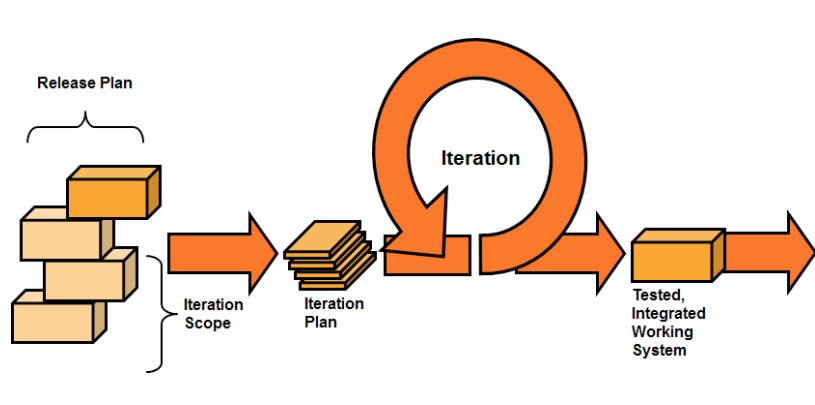
\includegraphics[scale=0.5]{img/agili/agili.png}
      \caption{Rappresentazione grafica di un metodo agile.}
      \label{fig:agili}
\end{figure}
Potenzialmente dopo un'iterazione si può arrivare ad un prodotto che può essere
messo in produzione. Dopo ogni rilascio si raccolgono feedback per poter rivalutare
i requisiti e migliorare il progetto. Si hanno quindi aspetti comuni nei metodi
agili e nel loro processo:
\begin{itemize}
      \item \textbf{Enfasi sul team}: sulla sua qualità e sulla sua selezione.
      \item \textbf{Team è self organizing}: si da importanza ai vari membri
            del team dato che non esiste un manager, ma è il team stesso a
            gestire lo sviluppo.
      \item \textbf{Enfasi al pragmatismo}: focalizzandosi su una documentazione
            efficace evitando di produrre documenti inutili e difficili da
            mantenere.
      \item \textbf{Enfasi sulla comunicazione diretta}: sostituendo i documenti
            suddetti con meeting e riunioni periodiche.
      \item \textbf{Enfasi sull'idea che nulla sia definitivo}: la perfezione non
            deve essere seguita fin da subito ma saranno gli step a portare al
            raggiungimento di una perfezione finale.
      \item \textbf{Enfasi sul controllo costante}: della qualità del prodotto,
            anche tramite:
            \begin{itemize}
                  \item \textbf{Continuous testing}: grazie al quale un insieme
                        di test viene eseguito in modo automatico dopo ogni modifica.
                  \item \textbf{Analisi statica e dinamica} del codice al fine
                        di trovare difetti nello stesso.
                  \item \textbf{Refactoring}.
            \end{itemize}
\end{itemize}
I metodi agili sono molto “elastici” e permettono la facile definizione di nuovi
metodi facilmente adattabili al singolo progetto.
\section{Scrum}
Uno dei più famosi, tra i vari metodi agili, è \textbf{scrum} (\ref{fig:scrum}).
\begin{figure}[!ht]
      \centering
      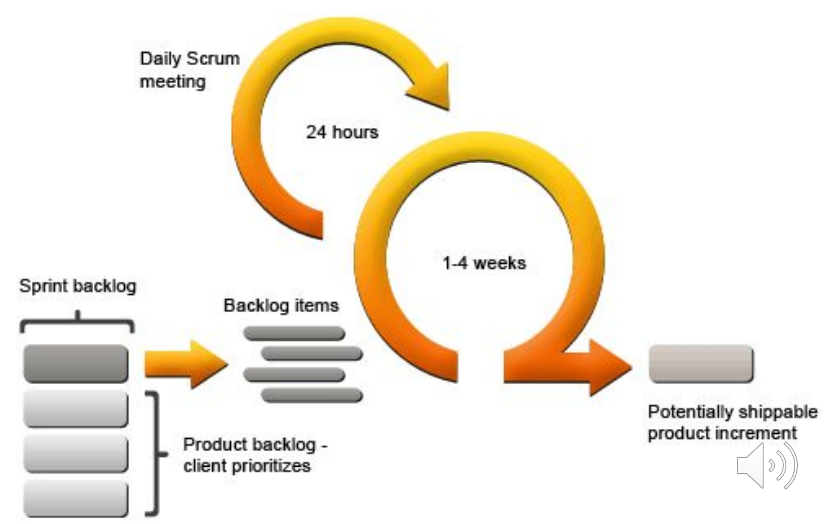
\includegraphics[scale=0.5]{img/agili/scrum.png}
      \caption{Rappresentazione grafica del processo scrum}
      \label{fig:scrum}
\end{figure}
In questo caso la parte di sviluppo e iterazione prende il nome di \textbf{sprint}
ed ha una durata variabile, tra una e quattro settimane, per avere un rilascio
frequente e una veloce raccolta di feedback. I requisiti sono raccolti nel cosiddetto
\textbf{product backlog}, con priorità basata sulla base delle indicazioni del
committente. Ad ogni sprint si estrae dal product backlog lo \textbf{sprint backlog},
ovvero il requisito (o i requisiti) da implementare nello sprint. Lo sprint backlog
viene analizzato nel dettaglio producendo i vari \textbf{backlog items}, ovvero
le singole funzionalità che verranno implementate nello sprint. Si ottiene quindi
di volta in volta un pezzo di prodotto finale, testato e documentato. Durante le
settimane di sprint si effettua anche un meeting giornaliero utile per mantenere
alti i livelli di comunicazione e visibilità dello sviluppo. Durante il meeting
ogni sviluppatore risponde a tre domande:
\begin{enumerate}
      \item Cosa è stato fatto dall'ultimo meeting?
      \item Cosa farai fino al prossimo meeting?
      \item Quali sono le difficoltà incontrate?
\end{enumerate}
L'ultimo punto permette la cooperazione tra team members, consci di cosa ciascuno
stia facendo. Durante il processo scrum si hanno quindi tre ruoli:
\begin{enumerate}
      \item \textbf{Product owner}: committente che partecipa tramite feedback
            e definizione dei requisiti.
      \item \textbf{Team} che sviluppa.
      \item \textbf{Scrum master}: che controlla la correttezza di svolgimento
            del processo scrum.
\end{enumerate}
Lo scrum master interagisce in ogni fase, ognuna delle quali viene guidata
tramite meeting:
\begin{itemize}
      \item \textbf{Sprint planning meeting}: ad inizio sprint per pianificare
            cosa fare nello sprint.
      \item \textbf{Daily scrum meeting}: il meeting giornaliero per aggiornare
            tutti i membri del team su quello che ciascuno sta facendo e deve
            essere il più breve possibile.
      \item \textbf{Sprint review meeting}: in uscita dallo sprint per lo studio
            dei risultati e analisi di quello che è stato sviluppato.
      \item \textbf{Sprint retrospective meeting}: in uscita dallo sprint per lo
            studio, tra i membri del team, di eventuali miglioramenti da apportare
            al processo Scrum e allo sviluppo del prodotto.
\end{itemize}
Spesso nelle singole iterazioni si utilizza la metodologia di sviluppo basata
sull'\textbf{extreme programming}, ovvero:
\begin{itemize}
      \item Planning delle attività
      \item Short release
      \item Simple design
      \item Refactoring
      \item Test first design
      \item Pair programming
      \item Collective Ownership
      \item Continuous Integration
      \item 40-h week
      \item On-site customer
      \item Coding standard
      \item Open workspace
\end{itemize}
\section{Extreme Programming}
Un altro tipo di metodo agile è l'\textbf{extreme programming}, ormai poco usato.
I requisiti prendono i nomi di stories, delle narrazioni in cui l'attore
(futuro utente del sistema) cerca di svolgere un compito. Vengono scelte quindi
stories per la prossima iterazione, dove si hanno testing e revisione continua.
Le release di ogni iterazione vengono catalogate per importanza (con anche la
solita collezione di feedback).
\chapter{DevOps}
Negli ultimi tempi si è sviluppato un altro metodo, chiamato DevOps, dove anche
la parte di \textbf{operation} deve essere agile: il rilascio in produzione e il
deployment devono essere agili quanto lo
sviluppo.

Nel DevOps (\ref{fig:devops}) i team di sviluppo e operation sono indipendenti
tra loro, diminuendo il costo di impegno necessario al team di sviluppo per la
parte di deployment, la quale viene resa anche più sicura grazie alla diminuzione
dell'intervento umano in favore di automazioni. Inoltre, avendo i due team dei
tempi di lavoro diversi, si riesce a prevenire ritardi causati dalla non
organicità delle operazioni.
\begin{figure}[!ht]
      \centering
      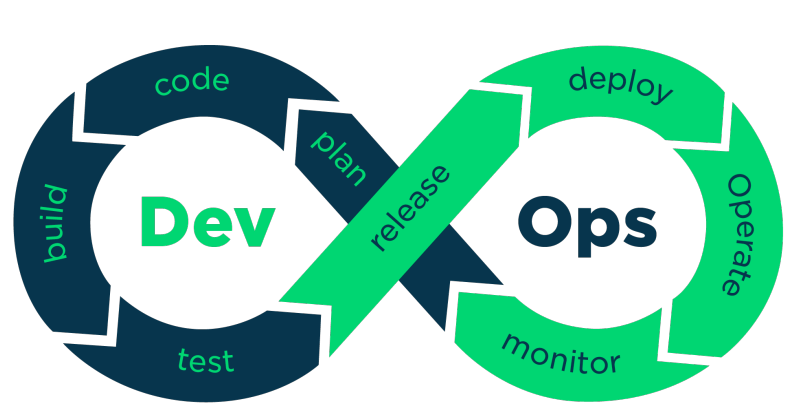
\includegraphics[scale=0.5]{img/devops/devops.png}
      \caption{Rappresentazione del lifecycle di DevOps}
      \label{fig:devops}
\end{figure}
DevOps promuove la collaborazione tra i due team al fine di ottenere una sorta
di team unico che curi sia sviluppo che operation. DevOps include quindi diversi
processi che vengono automatizzati:
\begin{itemize}
      \item Continuous Development
      \item Continuous Integration
      \item Continuous Testing
      \item Continuous Deployment
      \item Continuous Monitoring
\end{itemize}
Con DevOps il feedback arriva in primis dal software inoltre il focus viene
spostato sui processi automatici. Nel DevOps si introducono nuovi ruoli:
\begin{itemize}
      \item Il \textbf{DevOps Evangelist}, simile allo scrum master, supervisiona
            l'intero processo di DevOps.
      \item L'\textbf{automation expert}, dedicato a curare gli aspetti di
            automatismo.
      \item Un \textbf{Security Engineer}
      \item Un \textbf{Software Developer}, nonché Tester
      \item Un \textbf{Quality Assurance} che verifica la qualità del prodotto
            rispetto ai requisiti.
      \item Un\textbf{ Code Release Manager} che si occupa sull'infrastruttura e
            sul deploy della release
\end{itemize}
DevOps si basa su sei principi base:
\begin{enumerate}
      \item \textbf{Customer-Centric Action}, ovvero il committente è al centro
            dell'azione
      \item \textbf{End-To-End Responsibility}, ovvero il team gestisce interamente
            il prodotto, avendone responsabilità totale
      \item \textbf{Continuous Improvement}, ovvero cercare continuamente di
            migliorare senza sprechi il prodotto finale e i servizi.
      \item \textbf{Automate everything}, ovvero cercare di automatizzare l'intera
            infrastruttura di processo, dalle attività di testing e integrazione
            fino ad arrivare alla costruzione della release e del deployment.
      \item \textbf{Work as one team}, ovvero unificare tutti gli aspetti sotto un
            unico team o comunque con due team che collaborano fortemente come se
            fossero uno.
      \item \textbf{Monitor and test everything}, ovvero testare e monitorare
            costantemente il prodotto
\end{enumerate}
Il quarto e il sesto punto sono i due punti tecnici principali.
\section{Build, Test e Release}
Bisogna pensare a questi step in ottica di automatismo vicina al DevOps.
Innanzitutto bisogna introdurre i sistemi di version control (Git) un sistema di
version control distribuito, dove ogni utente ha una copia della repository
(con la storia dei cambiamenti), con la quale interagisce tramite commit e update.
Esiste poi una repository lato server per permettere di condividere i vari
cambiamenti tramite sincronizzazione.
\begin{figure}[!ht]
      \centering
      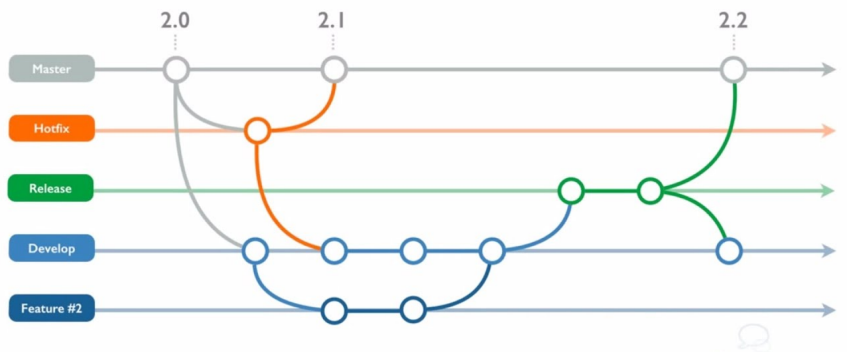
\includegraphics[scale=0.5]{img/devops/git.png}
      \caption{Struttura ideale di un repository git}
      \label{fig:git}
\end{figure}
Lo sviluppo su multi-branch si collega alle operazioni di verifica che possono
essere attivate automaticamente a seconda dell'evoluzione del codice su ogni branch.
Avendo ogni branch una precisa semantica possiamo definire precise attività di
verifica, corrispondenti a pipelines precise, solitamente innescate da un push di
codice su un certo branch, in modo sia automatico che manuale.
Le pipeline vengono attivate in fase di test di un componente, in fase di creazione
di un sottosistema, di assembramento di un sistema intero o di deployment in
produzione. Si hanno quindi quattro fasi:
\begin{enumerate}
      \item \textbf{component phase}
      \item \textbf{subsystem phase}
      \item \textbf{system phase}
      \item \textbf{production phase}
\end{enumerate}
Spesso le pipelines sono usate come \textbf{quality gates} per valutare se un push
può essere accettato in un certo branch. Una pipeline può essere anche regolata
temporalmente, in modo che avvenga solo ad un certo momento della giornata.
\subsection{Component phase e Subsystem phase}
Dove il focus è sulla più piccola unità testabile che viene aggiornata che non
può essere eseguita senza l'intero sistema. In tal caso si può fare:
\begin{itemize}
      \item Code review
      \item Unit testing
      \item Static code analysis
\end{itemize}
Un cambiamento può anche essere testato nell'ambito del sottosistema di cui fa
parte, in tal caso si hanno anche check di prestazioni e sicurezza. Il servizio
però potrebbe essere da testare in isolamento rispetto ad altri servizi, usando
quindi dei mocks o degli stubs, ovvero creando degli alter ego dei servizi mancanti
in modo che il servizio da testare possa funzionare.
\subsection{System phase}
In questo caso si testa l'intero sistema che viene “deployato” in ambiente di test.
Si hanno:
\begin{itemize}
      \item Integration tests
      \item Performance tests
      \item Security tests
\end{itemize}
Tutti test che richiedono l'interezza del sistema e sono spesso molto dispendiosi e
quindi bisogna regolare la frequenza di tali test in molti casi.
\subsection{Production phase}
Questa fase è legata alla necessità di creare gli artefatti che andranno
direttamente “sul campo”, ovvero il deployment in produzione. In tale fase potrebbe
essere necessario creare container o macchine virtuali. Si hanno dei check molto
veloci sugli artefatti finali, dando per assodato che la qualità del codice sia già
stata testata. Si hanno quindi strategie anche di deployment incrementale, per
cui esistono più versioni del software contemporaneamente con diversa accessibilità
per gli utenti finali. In tal caso si usano anche vari tool di monitor. Si hanno
anche eventualmente tecniche di zero downtime.

Fasi diverse corrispondono a branch diversi
\section{Deploy, Operate e Monitor}
Si studia l'evoluzione automatica del software da una versione all'altra in
produzione. Avanzare di versione in modo naive e istantaneo è troppo rischioso e
quindi spesso non attuabile. Si ha quindi un insieme di tecniche che si basano
in primis sull'evoluzione incrementale.

Tali tecniche si distinguono in base alla dimensione su cui sono incrementati:
\begin{itemize}
      \item \textbf{Incremental with reference to users}: Dark launching, Canary
            releases (and User Experimentation), ovvero legata agli utenti esposti
            alla nuova release.
      \item \textbf{Incremental with reference to requests}: Gradual upgrades/rollout,
            ovvero legata alle richieste per la nuova release.
      \item \textbf{Incremental with reference to components/replicas}: Rolling
            upgrade, incentrata sulle componenti che vengono aggiornate.
      \item \textbf{Non-incremental with backups}: Green/blue deployment,
            Rainbow deployment, non incrementali ma che offrono comunque un backup
            di sicurezza.
\end{itemize}
Tali schemi possono essere usati in un contesto DevOps. Per studiare la prima
tipologia (Incremental with reference to users) abbiamo:
\begin{itemize}
      \item \textbf{Dark launching}: In tale schema l'update è esposto solo ad una
            parte della popolazione, per la quale viene effettuato il deployment
            per studiare gli effetti ed eventuali modifiche e migliorie al software,
            che infine verrà deployato per il resto della popolazione in modo
            comunque incrementale fino a che l'intera popolazione godrà della feature.
      \item \textbf{Canary releases}, che studia l'impatto di update relativi al
            backend
\end{itemize}

Tali schemi spesso sono usati di pari passo per le varie sezioni del software,
nonché possono essere usati in modo intercambiabile.

Collegato a questi schemi si ha l'approccio basato sull'\textbf{user experimentation},
che non è un reale schema di gestione dell'evoluzione del software ma è comunque
correlato agli schemi sopra descritti. In questo approccio si studiano diverse
varianti del sistema e il loro impatto esponendole agli utenti, cercando di capire
per l'utente cosa sia meglio e come. Si hanno quindi più release diverse, per
parti di popolazione comparabili, tra le quali si sceglierà la migliore.

Per la seconda tipologia (Incremental with reference to requests) si ha una
divisione a seconda delle richieste fatte dagli utenti, detto \textbf{gradual rollout}.
Si ha quindi un load balancer che permette la coesistenza di due versioni, una
nuova e una vecchia, dello stesso servizio. In modo graduale, partendo da pochissime,
si passano le richieste alla versione nuova per poter studiare e testare la nuova
versione. Alla fine tutto il traffico sarà diretto verso la nuova versione, mentre
la vecchia verrà dismessa.

Per la terza tipologia (Incremental with reference to components/replicas),
si ha lo schema del \textbf{rolling upgrade}, dove l'upgrade non riguarda un
singolo upgrade ma tanti componenti di un sistema distribuito, verificando efficacia
di ogni singolo update tramite il continuous monitoring prima di effettuare l'upgrade
di un'altra componente. La stessa idea si applica anche a diverse versioni dello
stesso prodotto, aggiornandone una prima e poi le altre progressivamente.

Per la quarta tipologia (Non-incremental with backups) si ha il
\textbf{blue/green deployment}, dove vengono isolate due copie della stessa
infrastruttura, dove una ospita la versione nuove l'altra la vecchia. Un router
ridireziona le richieste degli utenti verso le due unità e quella che ospita la
nuova versione subirà le solite operazioni di test che, se superate, porteranno
il router a direzionare verso quella unità, ignorando la vecchia. Se ci sono problemi
si fa rollback alla vecchia unità che rimane come backup. Questo schema può essere
generalizzato nel rainbow deployment dove il momento di coesistenza tra le due
versioni viene prolungato al fine che vecchie richieste che richiedono una lunga
elaborazione vengano elaborate dall'unità vecchia mentre le nuove dall'unità nuova.

In ogni caso le applicazioni devono essere costruite per supportare tutti questi
schemi di deployment.
\subsection{Deployable units}
Il caso più tipico in merito alle unità dove fare deployment è il mondo del cloud,
con unità virtualizzate e virtual machine (VM), dove magari ogni servizio vive in
una diversa VM. Si hanno diversi casi in merito a questo tipo di deployment:
\begin{itemize}
      \item \textbf{Cloud basato su VMs}, dove si ha un'infrastruttura gestita dal
            cloud provider che gestisce l'hardware e l'hypervisor. Ogni VM, che
            sono le nostre unità di deployment, ha un sistema operativo arbitrario
            che lavora con l'hardware mostrato dall'hypervisor. Ogni VM avrà una
            o più applicazioni e fare deployment porterà all'update di una o più
            VM. In alcuni casi si fa deployment di intere VM e in altri si modifica
            il software di una VM già in esecuzione. L'ambiente cloud solitamente
            è multi-tenant, ovvero su una piattaforma unica di un provider si
            hanno più VM di diverse organizzazioni.
            Una VM è grossa in quanto contiene un sistema operativo intero e la loro
            gestione può quindi essere difficoltosa.
      \item \textbf{Cloud basato su containers} che risolvono il problema della
            grandezza delle VM. In questo caso lo schema è il medesimo ma si ha
            un container engine al posto dell'hypervisor e ogni container non
            contiene l'intero sistema operativo ma solo il minimo necessario al
            funzionamento dell'applicazione. In questo caso lo schema di update
            spesso consiste nel distruggere e ricreare i singoli containers.
            Anche qui si ha un contesto multi-tenant.
      \item \textbf{Bare metal}, dove i provider offrono direttamente risorse
            hardware, guadagnando prestazioni ma aumentano anche i costi economici,
            che vengono comunque gestite dal cloud provider. Non si ha virtualizzazione
            ma accesso diretto alle risorse su cui fare deployment. Questa è una
            soluzione tipicamente single-tenant.
      \item \textbf{Server dedicati}, un metodo ormai superato con difficoltà causate
            dall'uso di script, shell e connessione ftp completamente autogestiti
            dall'organizzazione e non da un provider.
\end{itemize}
Il deployment “stile cloud” non è comunque l'unico possibile.
\subsection{Monitor}
In ambiente cloud ci sono tante soluzioni per il monitoring, ad esempio lo stack
di ELK, formato da:
\begin{itemize}
      \item Elasticsearch
      \item Logstash
      \item Kibana
\end{itemize}
I dati, ad esempio log o metriche d'uso hardware, vengono raccolti e passano da
Logstash, finendo in un database, per la memorizzazione di time series (serie
temporali) di dati (questo in primis per le metriche d'uso che per i log), gestito
da Elasticsearch e venendo visualizzati da una dashboard grafica, gestita da
Kibana. Si ha quindi un ambiente di continuous monitoring.
\subsection{DevOps tools}
Ogni step del DevOps è gestito tramite moderne tecnologie e tools, con varie
alternative per ogni fase (per questo servono figure esperte per ogni step).

\chapter{Risk management}
\section{Definizione del rischio}
\begin{definizione}[\textbf{Risk management}]
    Il \textbf{risk management} è la disciplina che si occupa di identificare,
    gestire e potenzialmente eliminare i rischi prima che questi diventino un
    problema per il successo del progetto.
\end{definizione}
\begin{definizione}[\textbf{Rischio}]
    Definiamo \textbf{rischio} come la possibilità che ci sia un danno.
\end{definizione}
\begin{definizione}[\textbf{Risk exposure}]
    Definiamo \textbf{risk exposure} come una grandezza, per calcolare quanto
    un progetto sia esposto ad un rischio. Viene calcolato come:
    \begin{equation}
        RE = P(UO) \cdot L(UO)
    \end{equation}
    dove:
    \begin{itemize}
        \item $P(UO)$: è la probabilità di un unsatisfactory outcome (UO), ovvero
              la probabilità che effettivamente un danno sia prodotto.
        \item $L(UO)$: è l'entità del danno stesso, ovvero è la perdita per le
              parti interessate se il risultato non è soddisfacente.
    \end{itemize}
    Tanto più un rischio è probabile e tanto più il rischio crea un danno, di
    conseguenza cresce il risk exposure.
\end{definizione}
\begin{definizione}[\textbf{Outcome unsatisfactory}]
    Definiamo \textbf{outcome unsatisfactory} come un risultato negativo che
    riguarda diverse aree:
    \begin{itemize}
        \item L'area relativa all'\textbf{esperienza degli utenti}, con un progetto che
              presenta le funzionalità sbagliate. In questo caso se i problemi sono
              gravi si hanno alti rischi che portano al fallimento del prodotto.
        \item L'area relativa agli \textbf{sviluppatori}, con rischi che possono riguardare
              superamento del budget oppure prolungamenti delle deadlines.
        \item L'area riguardante i \textbf{manutentori}, con rischi che impattano nella
              qualità bassa di software e hardware.
    \end{itemize}
\end{definizione}
Se abbiamo un rischio che produce un outcome unsatisfactory il primo elemento su
cui soffermarsi è lo studio degli eventi che abilitano il rischio, detti
\textbf{risk triggers}.

Possiamo distinguere due principali classi di rischio:
\begin{enumerate}
    \item \textbf{Process-related risks}: rischi con impatto negativo sul processo
          e sugli obiettivi di sviluppo.
    \item \textbf{Product-related risks}: rischi con impatto sul prodotto e su
          obiettivi del sistema funzionali o meno, come fallimenti riguardanti
          la qualità del prodotto o la distribuzione dello stesso.
\end{enumerate}
Entrambe le classi possono portare al fallimento del progetto e quindi vanno
gestite entrambe.
\section{Risk Management}
Bisogna quindi imparare a gestire i rischi. Per fare ciò si utilizza un processo
strutturato in due fasi:
\begin{enumerate}
    \item \textbf{Risk Assessment}: in questa fase si vanno a valutare i rischi
          attraverso:
          \begin{itemize}
              \item \textbf{Risk Identification}: fase di identificazione dei
                    rischi.
              \item \textbf{Risk Analysis}: l'analisi dei rischi identificati
                    nella fase precedente tramite calcolo del \textit{risk
                        exposure} e studio dei \textit{triggers}.
              \item \textbf{Risk Prioritization}: si vanno a definire delle
                    priorità nei rischi analizzati, in modo da concentrarsi sui
                    più pericolosi per poi passare a quelli meno pericolosi.
          \end{itemize}
          Alla fine di questa fase, si produce una lista ordinata sulla pericolosità
          dei rischi.
    \item \textbf{Risk Control}: consiste nel risk management planning, producendo
          piani di controllo di due tipi:
          \begin{enumerate}
              \item \textbf{Piani di management}: per la gestione del rischio
                    prima che si verifichi.
              \item \textbf{Piani di contingency}: per il contenimento di rischi
                    divenuti realtà qualora il piano di management fallisca,
                    sapendo cosa fare a priori in caso di emergenza.
          \end{enumerate}
          Si hanno quindi due sotto-fasi per i due tipi di piani:
          \begin{enumerate}
              \item \textbf{Risk monitoring}.
              \item \textbf{Risk resolution}.
          \end{enumerate}
\end{enumerate}
Queste due fasi vengono ciclicamente ripetute durante il ciclo di vita dello
sviluppo di un software.
\subsection{Risk identification}
In questa fase, si studia come identificare i rischi. Tale operazione è legata
alle competenze degli analisti. Un modo comune di realizzare questa operazione è
mediante l'uso delle \textbf{check-list}, liste che includono un insieme di rischi
plausibili comuni a molti progetti. L'analista scorre tale lista cercando rischi
che possono essere applicati al progetto in analisi.

Alcuni rischi possono verificarsi sempre ma va preso in considerazione solo per
motivi specifici identificabili nel mio progetto. Si hanno altri metodi per
identificare i rischi:
\begin{itemize}
    \item \textbf{Riunioni di confronto}, \textbf{brainstorming} e \textbf{workshop}.
    \item Confronto con altre \textbf{organizzazioni} e con altri \textbf{prodotti}.
\end{itemize}
\subsection{Risk analysis}
L'analisi dei rischi viene realizzata sfruttando l'esperienza e valutando le
reali probabilità che un rischio diventi reale. Come per la fase precedente, si
hanno degli schemi su cui basarsi:
\begin{itemize}
    \item \textbf{modelli di stima dei costi}
    \item \textbf{modelli delle prestazioni} basati su simulazioni, prototipi e analogie con altri progetti
    \item \textbf{check-list}
\end{itemize}

L'analisi dei rischi può anche comportare lo studio delle decisioni da prendere
al fine di minimizzare il risk exposure, scegliendo o meno tra varie opzioni,
scegliendo in modo guidato dai rischi. 

A tal fine si usano i \textbf{decision tree} nei quali la radice rappresenta il problema.
Si hanno di volta in volta i vari scenari, con le stime di probabilità di trovare
un errore critico, di fallimento, di non avere errori. Tali
probabilità verranno usate per il calcolo del risk exposure insieme ad un
quantificatore di $L(UO)$, spesso pari all'effettivo costo che conseguirebbe al
risultato ottenuto. Infine, i vari risk exposure di ogni caso vengono sommati per
ottenere il risk exposure finale. 

Si può fare un'\textbf{analisi di sensitività}
cambiando le percentuali o i costi al fine di capire come comportarsi, riducendo
al minimo il danno e il rischio.

\begin{esempio}[Decision tree]
    Vediamo ora un esempio di come utilizzare un albero di decisione per effettuare
    l'analisi di un rischio figura \ref{fig:tree}.
    \begin{figure}[!ht]
        \centering
        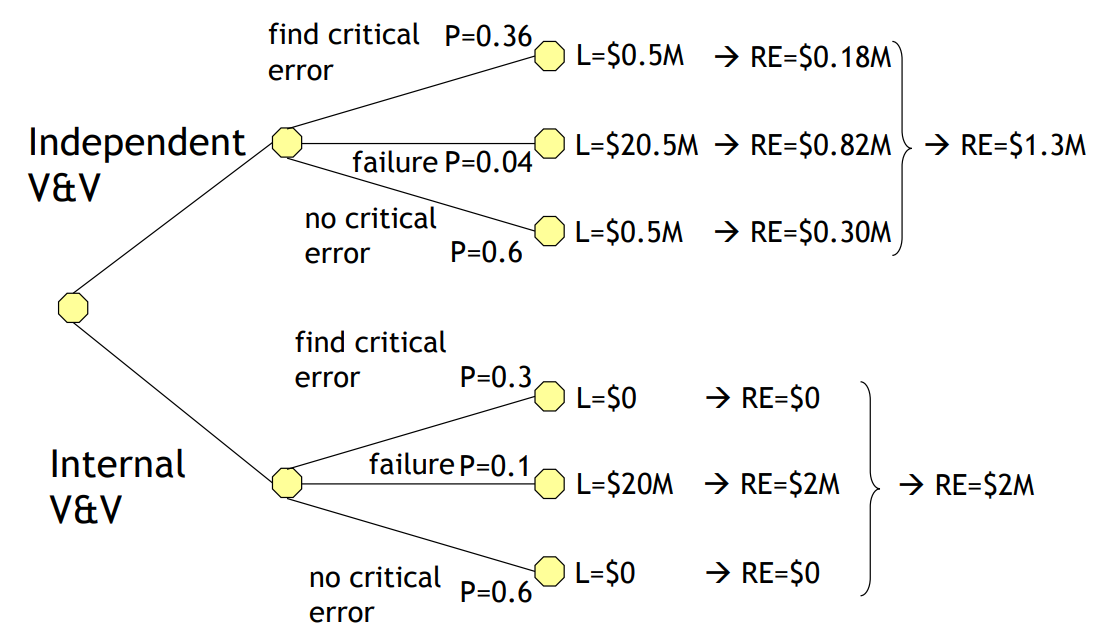
\includegraphics[width=0.5\textwidth]{img/risk/tree.png}
        \caption{Decision tree}
        \label{fig:tree}
    \end{figure}
\end{esempio}

Per ragionare sulle cause dei rischi usiamo il cosiddetto \textbf{risk tree}. Questo
albero ha come radice il rischio. Ogni nodo, detto \textbf{failure node}, è un
evento che si può scomporre in altri eventi, fino alle foglie. La scomposizione
è guidata da due tipi di nodi link:
\begin{enumerate}
    \item \textbf{and-node}: dove i figli di tali nodi sono eventi legati dal un
          and.
    \item \textbf{or-node}: dove i figli di tali nodi sono eventi legati dal un
          or.
\end{enumerate}
\begin{esempio}[Risk tree]
    Vediamo ora un esempio di risk tree figura \ref{fig:risk-tree}.
    \begin{figure}[!ht]
        \centering
        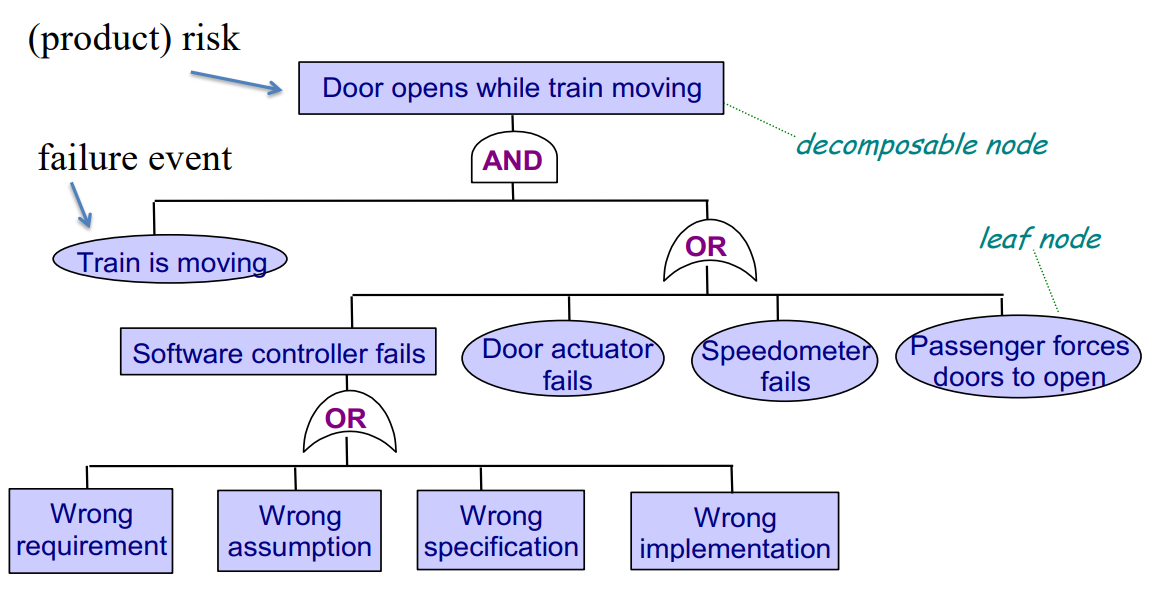
\includegraphics[width=0.5\textwidth]{img/risk/risktree.png}
        \caption{Risk tree}
        \label{fig:risk-tree}
    \end{figure}
\end{esempio}
Nodi $and/or$ vengono rappresentati tramite i simboli delle porte logiche. Dato un
risk tree cerco le combinazioni di eventi atomici che possono portare al rischio.
Per farlo si esegue la \textbf{cut-set tree derivation}, ovvero, partendo dalla radice, si
riporta in ogni nodo la combinazione di eventi che possono produrre il fallimento
e si vanno a calcolare le varie combinazioni degli eventi foglia. Praticamente si
deriva un insieme di eventi non scomponibili sulle combinazioni dell'and.

\begin{esempio}[Cut-set tree]
    Vediamo ora un esempio di cut-set tree figura \ref{fig:cut-set-tree}.
    \begin{figure}[!ht]
        \centering
        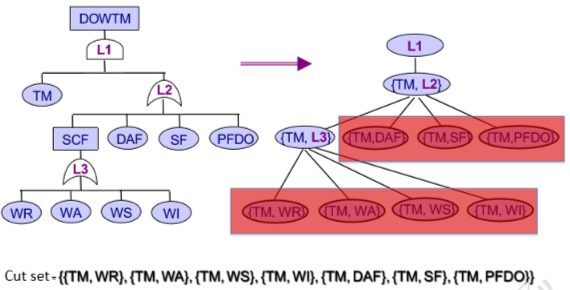
\includegraphics[width=0.5\textwidth]{img/risk/cut-set_tree.png}
        \caption{Cut-set tree}
        \label{fig:cut-set-tree}
    \end{figure}
\end{esempio}

\subsection{Risk prioritization}
Bisogna capire quali rischi sono più importanti di altri. Per farlo si pongono i
valori di $P(UO)$ e $L(UO)$ in un range, per esempio, da 1 a 10, ricalcolando il
risk exposure. Una volta fatto si lavora in base al risk-exposure.

\begin{esempio}[Risk-exposure analysis]
    Vediamo ora un esempio del piano cartesiano di analisi della risk-exposure in
    figura \ref{fig:risk-exposure-analysis}. In questo modo è possibile identificare
    delle regioni del grafico con valori particolari di risk-exposure.
    \begin{figure}[!ht]
        \centering
        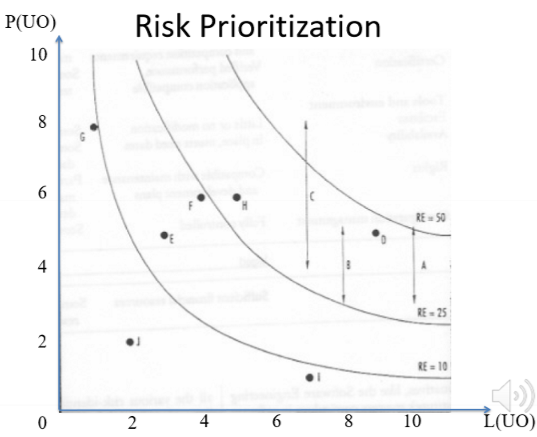
\includegraphics[width=0.5\textwidth]{img/risk/risk-prioritization.png}
        \caption{Risk-exposure analysis}
        \label{fig:risk-exposure-analysis}
    \end{figure}
\end{esempio}

Si procede disegnando i dati su un piano con $P(UO)$ sull'asse delle y e $L(UO)$
su quello  delle x e posizionandogli eventi su tale piano. Qualora i valori di RE siano
in un range, allora si rappresentano le RE minima e massima. 
Una volta rappresentati gli eventi, posso utilizzare delle curve per
identificare zone di rischio diverse in base al risk exposure in modo da
classificare i vari eventi.

\subsection{Risk control}
Bisogna quindi capire come gestire i rischi. Per ogni rischio bisogna definire e
documentare un piano specifico indicante:
\begin{itemize}
    \item Cosa si sta gestendo.
    \item Come mitigare il rischio e quando farlo.
    \item Di chi è la responsabilità.
    \item Come approcciarsi al rischio.
    \item Il costo dell'approccio al rischio.
\end{itemize}
Anche in questo caso ci vengono incontro \textbf{liste} e \textbf{check-list} con le tecniche di risk
management più comuni in base al rischio specifico. Ci sono comunque strategie generali:
\begin{itemize}
    \item Abbassare la probabilità di realizzazione del rischio, lavorando sulla probabilità 
          dei triggers. ($P(UO) \to 0$)
    \item Lavorare sull'eliminazione del rischio. ($P(UO) = 0$)
    \item Lavorare sulla riduzione delle conseguenze del danno,
          non viene quindi ridotto il rischio. ($L(UO) \to 0$)
    \item Lavorare sull'eliminazione del danno conseguente al rischio. ($L(UO) = 0$)
    \item Lavorare sul mitigare le conseguenze di un rischio, diminuendo l'entità
          del danno. ($L(UO) \to 0$)
\end{itemize}
Bisogna anche studiare le \textbf{contromisure}, da scegliere e attivare in base
alla situazione. Si hanno due metodi quantitativi principali per ragionare
quantitativamente sulle contromisure:
\begin{enumerate}
    \item \textbf{Risk-reduction leverage}: dove si calcola quanto una certa
          contromisura può ridurre un certo rischio, utilizzando la seguente
          formula:
          \begin{equation}
              RRL(r, cm) = \frac{RE(r) - RE(\frac{r}{cm})}{cost(cm)}
          \end{equation}
          dove $r$ rappresenta il rischio, $cm$ la contromisura e $\frac{r}{cm}$
          la contromisura $cm$ applicata al rischio $r$.

          Calcolo quindi la differenza di risk exposure avendo e non avendo la
          contromisura e la divido per il costo della contromisura. La miglior
          contromisura è quella con il RRL maggiore, avendo minor costo e maggior
          efficacia dal punto di vista del risk exposure.
    \item \textbf{Defect detection prevention}: questo metodo confronta le varie
          contromisure, confrontando anche gli obiettivi del progetto, in modo
          quantitativo facendo un confronto indiretto, producendo matrici in cui
          si ragiona in modo indipendente sulle singole contromisure e sui singoli
          rischi ma confrontando anche in modo multiplo.

          Si ha un ciclo a tre step:
          \begin{enumerate}
              \item \textbf{Elaborare la matrice di impatto dei rischi} (\textit{risk
                        impact matrix}) \ref{fig:impact-matrix}: questa matrice
                    calcola l'impatto dei rischi sugli obiettivi del progetto.
                    I valori della matrice variano da 0, nessun impatto, a 1,
                    completa perdita di soddisfazione. Ogni rischio viene
                    accompagnato dalla probabilità $P$ che accada. Ogni obiettivo
                    è accompagnato dal peso $W$ che ha nel progetto.
                    \begin{figure}[!ht]
                        \centering
                        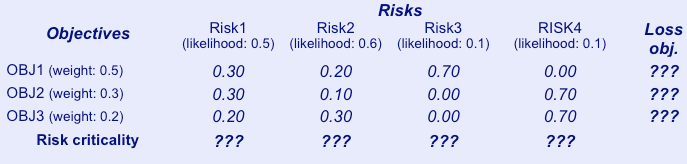
\includegraphics[width=0.5\textwidth]{img/risk/riskImpact.png}
                        \caption{Esempio di matrice di impatto dei rischi}
                        \label{fig:impact-matrix}
                    \end{figure}

                    La \textbf{criticità} di un rischio rispetto a tutti gli
                    obiettivi indicati:
                    \begin{equation}
                        \text{criticality}(r) = P(r) \cdot \sum_{obj}
                        (\text{impact\_matrix}[r, obj] \cdot W(obj))
                    \end{equation}
                    La criticità sale se sale l'impatto e se sale la probabilità
                    del rischio. Un altro dato è la \textbf{perdita} di raggiungimento
                    di un obiettivo qualora tutti i rischi si verificassero:
                    \begin{equation}
                        loss(obj) = W(obj) \cdot \sum_{r}
                        (\text{impact\_matrix}[r, obj] \cdot P(r))
                    \end{equation}
              \item \textbf{Elaborare contromisure efficaci per la matrice}:
                    \ref{fig:eff-matrix} si usa il fattore di criticità del
                    rischio. Viene prodotta una nuova matrice con colonne pari
                    ai rischi e righe pari alle contromisure. I valori saranno
                    le riduzioni di rischio di una contromisura $cm$ sul rischio
                    $r$. La riduzione va da 0, nessuna riduzione, a 1, rischio
                    eliminato.
                    \begin{figure}[!ht]
                        \centering
                        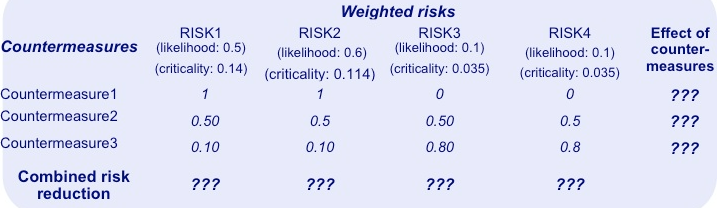
\includegraphics[width=0.5\textwidth]{img/risk/Effectiveness Matrix.png}
                        \caption{Esempio di matrice di efficacia delle contromisure}
                        \label{fig:eff-matrix}
                    \end{figure}

                    Possiamo calcolare la \textbf{combineReduction}, che ci dice
                    quanto un rischio viene ridotto se tutte le contromisure sono
                    attivate:
                    \begin{equation}
                        \text{combineReduction}(r) = 1 - \prod_{cm}(1 -
                        \text{reduction\_matrix}[cm, r])
                    \end{equation}
                    Un altro valore è l'\textbf{overallEffect}, ovvero l'effetto
                    di ogni contromisura sull'insieme dei rischi considerato:
                    \begin{equation}
                        \text{overallEffect}(cm) = \sum_{r} (\text{reduction\_matrix}[cm, r]
                        \cdot \text{criticality}(r))
                    \end{equation}
                    si avrà effetto maggior riducendo rischi molto critici.
              \item \textbf{Determinare il bilanciamento migliore tra riduzione
                        dei rischi e costo delle contromisure}.
                    Bisogna considerare anche il costo di ogni contromisura e
                    quindi si fa il rapporto tra effetto di ciascuna contromisura
                    e il suo costo e scegliendo il migliore.
          \end{enumerate}
\end{enumerate}
Il \textbf{contingency plan} viene attuato qualora il rischio si traduca in realtà.
Si passa quindi al risk monitoring/resolution. Queste due parti sono tra loro
integrate. I rischi vanno monitorati e all'occorrenza vanno risolti il prima
possibile. Tutte queste attività sono costose e si lavora su un insieme limitato
di rischi.
\chapter{Capability Maturity Model Integration}
Il \textbf{Capability Maturity Model Integration} (CMMI) che è un programma di
formazione e valutazione per il miglioramento a livello di processo gestito dal
CMMI Institute.

Bisogna prima introdurre il concetto di \textbf{maturità dei processi}. La
probabilità di portare a termine un progetto dipende dalla maturità del progetto
e la maturità dipende dal grado di controllo che si ha sulle azioni che si vanno
a svolgere per realizzare il progetto. Si ha quindi che:
\begin{itemize}
      \item Il progetto è \textbf{immaturo} quando le azioni legate allo sviluppo non sono
            ben definite o ben controllate e quindi gli sviluppatori hanno troppa
            libertà alzando la probabilità di fallimento.
      \item Il progetto è \textbf{maturo} quando le attività svolte sono ben definite,
            chiare a tutti i partecipanti e ben controllate. Si ha quindi un modo
            per osservare quanto si sta svolgendo e verificare che sia come
            pianificato, alzando le probabilità di successo e riducendo quelle di
            fallimento.
\end{itemize}
Risulta quindi essenziale ragionare sulla maturità del processo. Tale valore è
definito tramite un insiemi di livelli di maturità con associate metriche per
gestire i processi, questo è detto \textbf{Capability Maturity Model} (CMM). In
altri termini il modello CMM è una collezione dettagliata di best practices che
aiutano le organizzazioni a migliorare e governare tutti gli aspetti relativi al
processo di sviluppo.
\begin{center}
      \textit{Un processo migliore porta ad un prodotto migliore.}
\end{center}
Il modello CMMI è composto da:
\begin{itemize}
      \item \textbf{Process area}: che racchiude al suo interno una collezione di
            pratiche organizzate secondo obiettivi e riguarda una certa area del
            processo. Nel CMMI abbiamo 22 diverse process area. Ciascuna process
            area ha:
            \begin{itemize}
                  \item \textbf{Purpose statement}: descrive lo scopo finale
                        della process area stessa.
                  \item \textbf{Introductory notes}: descrivano i principali
                        concetti della process area.
                  \item \textbf{Related process area}: se utile, con la lista
                        delle altre process area correlate a quella corrente.
            \end{itemize}
      \item Le process area si dividono in due tipologie di obiettivi:
            \begin{enumerate}
                  \item \textbf{Specific goals}: ovvero gli obiettivi specifici
                        della singola process area in questione. All'interno di
                        ognuno abbiamo una serie di \textbf{specific practices},
                        ovvero quelle azioni che se svolte permettono di raggiungere
                        quell'obiettivo specifico e, a loro volta, tali pratiche
                        sono organizzate in:
                        \begin{itemize}
                              \item \textbf{Example work product}: elenchi di
                                    esempi di prodotti che possono essere generati
                                    attraverso l'adempimento delle pratiche.
                              \item \textbf{Subpractices}: descrizione dettagliata
                                    per l'interpretazione e l'implementazione.
                        \end{itemize}
                  \item \textbf{Generic goals}: gli obiettivi comuni a tutte
                        le process area. Questi obiettivi rappresentano quanto la
                        process area sia ben integrata e definita nel contesto
                        del processo ma questi criteri sono generali. All'interno
                        dei quali abbiamo una serie di \textbf{generic practices},
                        comuni a tutti, con le pratiche che devono essere svolte
                        per gestire positivamente una qualsiasi process area e,
                        a loro volta, tali pratiche sono organizzate in:
                        \begin{itemize}
                              \item \textbf{Generic practices elaborations}:
                                    ulteriori informazioni di dettaglio
                                    per la singola pratica.
                              \item \textbf{Subpractices}: descrizione
                                    dettagliata per l'interpretazione e
                                    l'implementazione.
                        \end{itemize}
                        Tra i principali generic goals (GG) abbiamo:
                        \begin{itemize}
                              \item \textbf{GG1}: raggiungere i specific goals,
                                    tramite l'esecuzione delle specific practices.
                              \item \textbf{GG2}: “ufficializzare” un managed
                                    process, tramite training del personale,
                                    pianificazione del processo, controllo dei
                                    work product etc$\dots$
                              \item \textbf{GG3}: “ufficializzare” un defined
                                    process, tramite la definizione rigorosa del
                                    progetto e la raccolta di esperienze legate
                                    al processo.
                        \end{itemize}
            \end{enumerate}
\end{itemize}
Per capire quanto un processo software è organizzato secondo questo standard
bisogna “mappare” quali goals e quali pratiche si stanno svolgendo e usare CMMI
non solo come \textit{ispirazione} ma come vero e proprio standard per definire
le azioni da svolgere nonché per confrontare il nostro operato e studiarlo
qualitativamente. Lo studio qualitativo mi permette di stabilire la maturità del
progetti, secondo un certo livello di compliance, detto CMMI level. Tale qualità
che può essere certificata da enti certificatori appositi.

Studiamo a fondo questi livelli di maturità e la loro codifica. Si hanno due
linee di sviluppo/miglioramento:
\begin{enumerate}
      \item \textbf{Capability levels} (CL): indica quanto bene si sta gestendo
            una particolare process area. Quindi per una singola process area mi
            dice quanto bene sto raggiungendo i generic goals.

            Il capability level ha valore compreso tra 0 e 3, estremi inclusi:
            \begin{itemize}
                  \item \textbf{Level 0} o \textbf{incomplete}: dove le pratiche
                        per una specifica process area sono state svolte
                        parzialmente o probabilmente non vengono svolte.
                  \item \textbf{Level 1} o \textbf{performed}: dove si eseguono
                        le pratiche e i vari specific goals sono soddisfatti. (GG1)
                  \item \textbf{Level 2} o \textbf{managed}: dove oltre alle
                        pratiche si ha anche una gestione delle attività stesse.
                        Si ha una policy per l'esecuzione delle pratiche. (GG2)
                  \item \textbf{level 3} o \textbf{defined}: dove l'intero processo
                        è ben definito secondo lo standard, descritto rigorosamente
                        e si ha un processo completamente su misura dell'organizzazione.
                        (GG3)
            \end{itemize}
            I capability levels di ciascuna process area possono essere rappresentati
            su un diagramma a barre, dove viene indicato il livello attuale e il
            profile target, ovvero il livello a cui quella process area deve arrivare.
      \item \textbf{Maturity levels} (ML): indica il livello di maturità raggiunto
            dall'intero processo di sviluppo, basandosi su tutte le process area
            attivate.

            Il Maturity level ha valore compreso tra 1 e 5:
            \begin{itemize}
                  \item \textbf{Level 1} o \textbf{initial}: dove si ha un processo
                        gestito in modo caotico.
                  \item \textbf{Level 2} o \textbf{managed}: dove si ha un processo
                        ben gestito secondo varie policy.
                  \item \textbf{Level 3} o \textbf{defined}: dove si ha un processo
                        ben definito secondo lo standard aziendale.
                  \item \textbf{Level 4} o \textbf{quantitatively managed}: dove
                        si stabiliscono obiettivi quantitativi per la qualità e
                        le performance del processo, in modo da poterli utilizzare
                        per la gestione.
                  \item \textbf{Level 5} o \textbf{optimizing}: dove grazie alle
                        informazioni raccolte ottimizzo il processo, in un'idea di
                        continuous improvement del progetto.
            \end{itemize}
\end{enumerate}
Il raggiungimento della \textbf{maturità del processo} quando si utilizza la rappresentazione a stadi
si ha quando il \textbf{maturity level} è 4 o 5. Il raggiungimento del \textbf{maturity level} 
4 implica l'implementazione dei \textbf{maturity level} 2, 3 e 4 in tutte le aree del proccesso. 
Allo stesso modo, il raggiungimento del \textbf{maturity level} 5 
implica l'implementazione di tutte le aree di processo per \textbf{maturity level} 
2, 3, 4 e 5.

Mentre, quando si utilizza la rappresentazione continua, si raggiunge un'elevata
maturità usando il concetto di stadiazione equivalente. La maturità che è
equivalente al \textbf{maturity level} 4 utilizzando lo staging equivalente
si raggiunge quando si raggiunge a \textbf{capability level} 3 per tutte le aree di
processo, ad eccezione dell'Organizational Performance Management (OPM) e Causal
Analysis and Resolution (CAR). L'elevata maturità, equivalente al 
\textbf{maturity level} 5 utilizzando una equivalente è raggiunta quando si raggiunge 
il \textbf{capability level} 3 per tutte le aree di processo.

Si possono confrontare CMMI e le pratiche agili. Ciò che viene svolto ai livelli
2 e 3 (con qualche piccolo adattamento) di maturity level si fa ciò che viene
fatto anche coi metodi agili. In merito ai livelli 4 e 5 di maturity level si hanno
pratiche che non rientrano nell'ottica dei metodi agili. Quindi un'organizzazione
può usare i metodi agili ed essere standardizzata rispetto CMMI raggiungendo
un maturity level 2 o 3. CMMI è quindi uno standard industriale con certificazioni
ufficiali.
\chapter{Requirements Engineering}
Quando si parla di \textbf{requirements engineering} (RE) di fatto ci si concentra
sulla comprensione di come una soluzione software si deve comportare per risolvere
un certo problema. In questo senso bisogna prima comprendere quale sia il problema
da risolvere e in quale contesto tale problema si verifica, per poter arrivare
ad una soluzione corretta ed efficacie a problemi reali. Bisogna ben comprendere
il problema, non si parla quindi della progettazione in se, ma del “cosa” deve
fare il software.

Vediamo ora l'analogia classica per spiegare il RE, il problema mondo e la soluzione
macchina. Si hanno:
\begin{itemize}
      \item Il \textbf{mondo}, con un problema derivante dal mondo reale, mondo
            stesso che produce tale problema che bisognerà risolvere con un calcolatore.
      \item La \textbf{macchina}, che bisogna sviluppare per risolvere il problema.
      \item \textbf{Requirements engineering} che si occupa di definire gli effetti
            della macchina sul problema del mondo e definire assunzioni e proprietà
            principali del mondo stesso.
\end{itemize}

Macchina e mondo possono condividere alcuni componenti, con la macchina che
modifica il mondo. Nel requirements engineering studiamo quindi il mondo, senza
definire come funziona internamente la macchina.

Quando si parla di requirements engineering è bene distinguere due elementi:
\begin{itemize}
      \item Ogni volta che prendiamo in considerazione un problema esiste sempre
            un \textbf{system-as-is}, ovvero un sistema preesistente che già risolve il
            problema. Si ha quindi sempre un sistema da cui partire.
      \item Esiste sempre un \textbf{system-to-be}, ovvero il sistema che si andrà
            a realizzare. In altre parole è il sistema quando la macchina/software ci
            opera sopra.
\end{itemize}

Studiare il system-as-is è essenziale per poter lavorare al system-to-be.
\begin{definizione}[\textbf{requirements engineering}]
      Il \textbf{requirements engineering} è, formalmente, un insieme di attività:
      \begin{itemize}
            \item Per esplorare, valutare, documentare, consolidare, rivisitare e
                  adattare gli obiettivi, le capacità, le qualità, i vincoli e le ipotesi
                  su un system-to-be.
            \item Basate sul problema sorto dal system-as-is e sulle nuove opportunità
                  tecnologiche.
      \end{itemize}
      L'output di queste attività è un documento di specifica dei requisiti con
      tutto ciò che soddisfa il sistema. Se l'output non è un singolo documento si
      ha una collezione di singoli requisiti, che nel metodo agile sono storie/cards
      e in altri metodi un repository centrale con un db condiviso contenete i
      vari requisiti.

      In ogni caso si ha un insieme di requisiti su come si deve comportare il
      sistema che si andrà a realizzare.
\end{definizione}

In un modello di sviluppo a cascata requirements engineering è una delle primissime
attività, subito dopo quelle di definizione del sistema e di business plan.

Per gli aspetti tecnici è probabilmente la prima attività svolta, occupandosi di
ottenere il giusto sistema da sviluppare, prima di design, implementazione ed
evoluzione software etc$\dots$ che si occupano di ottenere il software giusto,
sviluppandolo nel modo corretto.

Errare nel requirements engineering può portare ad un ottimo software che risolve
i problemi sbagliati oppure a un software che non risolve tutti i problemi che
dovrebbe risolvere. Sbagliare il requirements engineering è una causa di
fallimento del progetto.

Lavorare sui requirements non è semplice per diversi motivi:
\begin{itemize}
      \item Si deve ragionare su tante versioni del sistema come il system as-is,
            il system to-be e il system to-be-next, volendo essere lungimiranti per il
            comportamento del sistema, sapendo e prevedendo evoluzioni future.
      \item Si lavora in ambienti ibridi in un contesto che va compreso a fondo.
      \item Si hanno diversi aspetti funzionali, qualitativi e di sviluppo.
      \item Si hanno diversi livelli di astrazione, con obiettivi strategici a
            lungo termine di inserimento sul mercato e dettagli operazionali.
      \item Si hanno tanti stakeholders, quindi con diverse parti interessati di
            cui risolvere problemi e interessi con potenziali conflitti tra i vari
            stakeholders.
      \item Si hanno tante attività tecniche legate l'una con l'altra:
            \begin{itemize}
                  \item Conflict management
                  \item Risk management
                  \item Evaluation of alternatives
                  \item Prioritization
                  \item Quality assurance
                  \item Change anticipation
            \end{itemize}
\end{itemize}
\section{Tipi di requisiti}
Bisogna anche ragionare sui tipi di requisiti su cui si deve lavorare. Una prima
differenza si ha nel modo in cui sono scritti i requisiti. Si hanno quindi:
\begin{itemize}
      \item \textbf{Descriptive statements}: indicano dei requisiti non negoziabili,
            rappresentano dei comportamenti derivanti dalle leggi del mondo su cui
            lavora. Si ha quindi zero margine di modifica.
      \item \textbf{Prescriptive statements}: indicano requisiti negoziabili.
\end{itemize}

Entrambi sono importanti e vanno considerati. Si possono avere requisiti non ovvi,
o lo sono in un contesto specialistico e quindi spesso non ovvi a chi lavora
sul software, che magari nemmeno sa che esistono.

I requisiti possono inoltre differire per gli elementi che prendono in considerazione.
Posso avere requisti:
\begin{itemize}
      \item \textbf{System requirements}: come si comporta l'ambiente, per capirne
            il funzionamento.
      \item \textbf{Software requirements}: come si comporta il software
            nell'ambiente, studiando i cosiddetti shared fenomena.
\end{itemize}
ricordando che:
\begin{center}
      Sistema = Ambiente + Software \\ System requirements = Software requirements
      + Domain Properties + Assumption
\end{center}
I requisti comunque non riguardano mai il comportamento interno del software.
\newline Si hanno 3 dimensioni:
\begin{enumerate}
      \item \textbf{Dimensione del why}: si identificano, analizzano e rifiniscono
            i requisiti del system-to-be per affrontare le carenze analizzate del
            system-as-is, in linea con gli obiettivi di business, sfruttando le opportunità
            tecnologiche. Si hanno le seguenti difficoltà:
            \begin{itemize}
                  \item Acquisire conoscenza del dominio
                  \item Valutare opzioni alternative
                  \item Abbinare problemi-opportunità e valutarli in termini di implicazioni,
                        e rischi associati.
                  \item Gestire obiettivi contrastanti.
            \end{itemize}
      \item \textbf{Dimensione del what}: si identificano, analizzano e rifiniscono
            le funzionalità del system-to-be per soddisfare gli obiettivi individuati in
            base a vincoli basati su ipotesi realistiche sull'ambiente. Si hanno le seguenti difficoltà:
            \begin{itemize}
                  \item Identificare il giusto set di funzionalità.
                  \item Specificarle precisamente per essere comprese da tutte le parti.
                  \item Garantire la tracciabilità backward per gli obiettivi del sistema.
            \end{itemize}
      \item \textbf{Dimensione del who}: si assegna responsabilità per gli obiettivi,
            i servizi, i vincoli tra i componenti del system-to-be in base alle loro
            capacità e agli obiettivi del sistema, oltre i confini dell'ambiente software.
            La difficoltà è valutare opzioni alternative per decidere il giusto grado
            di automazione.
\end{enumerate}

I requisti che riguardano l'ambiente possono essere di due forme:
\begin{itemize}
      \item \textbf{Domain properties}: proprietà riguardanti l'ambiente, immutabili.
      \item \textbf{assumptions}: su come è fatto l'ambiente. Il software funzionerà
            solo negli ambienti che soddisfano quella certa assunzione. Se troppo
            restrittive possono portare al fallimento del progetto, che riguarderebbe
            pochissimi casi particolari.
\end{itemize}
\begin{definizione}[\textbf{Domain property}]
      Definiamo \textbf{domain property} come un descriptive statement sui problemi
      legati ai fenomeni del mondo (a prescindere da qualsiasi software-to-be).
      $\text{Domain property} \  \subseteq M \times C$ se leggi che non possono
      essere infrante.
\end{definizione}
Si ha che:
\begin{center}
      Software requirements = \textit{map}(System requirements, Software requirements,
      Domain property)
\end{center}

È utile quindi fare una distinzione per quanto concerne i requisiti del software.
Abbiamo due famiglie principali:
\begin{itemize}
      \item \textbf{Requisiti funzionali}, che indicano le funzionalità che un
            sistema (system-to-be) deve implementare, cosa deve essere in grado di fare.
            Non sono prevedibili prima di studiare il sistema.
      \item \textbf{Requisiti non funzionali}, che indicano delle qualità o dei
            vincoli sulle funzionalità e quindi sui requisiti funzionali. Questa famiglia
            di aspetti non funzionali è più o meno standard.
\end{itemize}

Per l'identificazione dei requisiti non funzionali si può utilizzare una
\textit{tassonomia}, riportata in figura \ref{fig:tasso}, dove si trovano organizzati
aspetti non funzionali tali per cui, dopo aver individuato le funzionalità posso
ricercare eventuali requisiti non funzionali.
\begin{figure}[!ht]
      \centering
      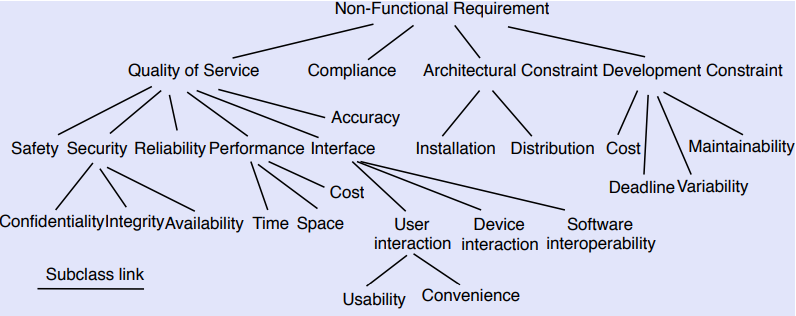
\includegraphics[width=0.5\textwidth]{img/requirements/tassonomia.png}
      \caption{Tassonomia dei requisiti non funzionali}
      \label{fig:tasso}
\end{figure}
Per alcuni tipi di progetti requisiti funzionali e non funzionali sono difficilmente
distinguibili, spesso mischiandosi.

Le intererazioni tra l'ambiente e sistema si possono effettuare secondo lo
schema \ref{fig:int-sistema-ambiente}.
\begin{figure}[!ht]
      \centering
      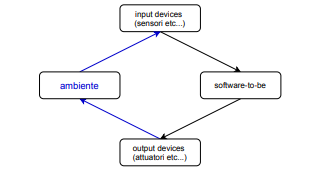
\includegraphics[width=0.5\textwidth]{img/requirements/interazione-sistema-ambiente.png}
      \caption{Schema delle interazioni tra sistema e ambiente}
      \label{fig:int-sistema-ambiente}
\end{figure}
Lo scambio di informazioni avviene mediante gli I/O device e 4 tipologie di variabili:
\begin{itemize}
      \item \textbf{input data} ($I$): variabili tra input device e sw-to-be
      \item \textbf{output results} ($O$): variabili tra sw-to-be e output device
      \item \textbf{controlled variables} ($C$): variabili tra output device e ambiente
      \item \textbf{monitored variables} ($M$): variabili tra ambiente e input device
\end{itemize}
I requisiti introdotti precedentemente sono in relazione con queste variabili.
$$\text{system requirements} \subseteq M\times C$$
$$\text{software requirements} \subseteq I\times O$$
$$\text{assunzioni} \subseteq M\times C\cup M\times I\cup C\times O$$
$$\text{Domain property}\subseteq M\times C$$
\section{Qualità dei requisiti}
Si hanno diversi aspetti di cui preoccuparsi nell'analisi dei requisiti. Si hanno
tante qualità indispensabili:
\begin{itemize}
      \item \textbf{Completezza}: è necessario descrivere tutti i requisiti rilevanti
            del progetto, identificando tutti i comportamenti del sistema e documentarli
            in modo adeguato. È una qualità virtualmente irraggiungibile in modo assoluto,
            non è infatti verificabile. Inoltre i requisiti variano al proseguire del
            progetto, interagendo anche con gli stakeholders, rendendo questo uno degli
            aspetti più difficili da studiare.
      \item \textbf{Consistenza}: i requisiti non devono presentare dei conflitti,
            dato l'elevato numero di requisiti è facile introdurre inconsistenze.
      \item \textbf{Non ambiguità}: tutto deve essere chiaro e non soggetto ad
            interpretazione.
      \item \textbf{Misurabilità}: non basato su interpretazioni vaghe ma su misure
            concrete e specifiche.
      \item \textbf{Fattibilità}: non si devono avere requisiti basati su
            funzionalità irrealizzabili.
      \item \textbf{Comprensibilità}.
      \item \textbf{Buona struttura}.
      \item \textbf{Modificabilità}: possibilità di avere il risultato mantenibile
            del tempo.
      \item \textbf{Tracciabilità}: individuando tutti gli artefatti ottenibili
            come conseguenza e tracciandoli. Si tracciano anche le dipendenze tra requisiti.
\end{itemize}
Vediamo quindi gli errori che si fanno quando si va ad identificare i requisiti:
\begin{itemize}
      \item \textbf{Omissioni}: non si riesce ad identificare qualche requisito.
            Anche un riconoscimento tardivo è un problema in quanto comporta la modifica
            del documento, non sempre facile.
      \item \textbf{Contraddizioni}: si presentano conflitti tra i requisiti.
      \item \textbf{Inadeguatezza}: requisiti che non sono adeguati per un determinato
            problema.
      \item \textbf{Ambiguità}: requisiti interpretabili.
      \item \textbf{Non misurabilità}: non si riesce a fornire una misura di certi
            requisiti, specialmente non funzionali, che comportano difficoltà di gestione,
            precludendo confronti etc$\dots$
\end{itemize}
Si hanno anche altri tipi di errore:
\begin{itemize}
      \item Essere troppo specifici nella definizione dei requisiti includendo
            anche comportamenti interni al software che non dovrebbero essere descritti
            in questa fase.
      \item Descrivere requisiti non implementabili considerando vincoli temporali
            o di costo.
      \item Descrivere requisti complessi da leggere.
      \item Avere poca struttura nella stesura dei requisiti, a livello visivo.
      \item Se si produce un documento bisogna evitare di fare riferimento a
            requisiti che non sono stati ancora descritti, ovvero evitando il forward
            reference.
      \item Evitare “rimorsi” di non aver definito nel momento giusto certi concetti
            che magari erano stati usati, senza definizione, precedentemente.
      \item Evitare la poco modificabilità del documento. È buona norma avere delle
            “costanti simboliche”, definite all'inizio, a cui fare riferimento nel documento,
            in modo che un'eventuale modifica si rifletta su tutto il documento.
      \item Evitare l'opacità/logica di fondo/razionale/motivazioni dei requisti,
            in modo che sia chiaro il perché esso è stato incluso, portando a mettere in
            discussione requisiti in realtà sensati a cui si arriverebbe comunque dopo
            ulteriore analisi, dopo aver perso ulteriore tempo.
\end{itemize}
\section{Il processo requirements engineering}
Si hanno 4 fasi a spirale (figura \ref{fig:spirale}):
\begin{figure}[!ht]
      \centering
      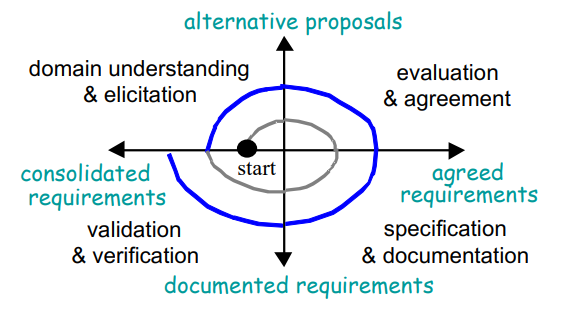
\includegraphics[width=0.6\textwidth]{img/requirements/spirale.png}
      \caption{Rappresentazione modello a spirale}
      \label{fig:spirale}
\end{figure}
\begin{enumerate}
      \item \textbf{Domain understanding} $\&$ \textbf{elicitation}: in questa fase
            si hanno due parti principali:
            \begin{itemize}
                  \item \textbf{Domain understanding}: in questa fase si ha  lo studio del
                        system-as-is in ottica di studio del dominio applicativo, studio del business
                        organizzazione che vuole il prodotto. Si studiano anche forze e debolezze del
                        system-as-is. Si studia il dominio applicativo per ottenere il miglior
                        system-to-be possibile. Inoltre, si identificano gli stakeholders del
                        progetto per poter capire a fondo interessi e fini.

                        Come output di questa fase si hanno le sezioni iniziali per la bozza di
                        proposta preliminare e il glossario dei termini.
                  \item \textbf{Requirements elicitation}: studio più approfondito nel mondo
                        attraverso un'ulteriore analisi dei problemi legati al system-as-is.
                        Inoltre, vengono identificati, grazie all'aiuto degli stakeholders:
                        \begin{itemize}
                              \item Opportunità tecnologiche.
                              \item Condizioni del mercato
                              \item Obiettivi di miglioramento
                              \item Vincoli, organizzativi e tecnici, del system-as-is
                              \item Alternative per raggiungere l'obiettivo e assegnare le responsabilità.
                              \item Scenari di ipotetica interazione software-ambiente
                              \item Requisiti del software
                              \item Assunzioni sull'ambiente
                        \end{itemize}
                        In in output si hanno ulteriori sezioni per la bozza di proposta preliminare.
            \end{itemize}
      \item \textbf{Evaluation} $\&$ \textbf{agreement}: si effettuano decisioni
            basate sull'interazione con i vari stakeholders, per poter valutare e decidere,
            avendo cambiamenti dei rischi in base a:
            \begin{itemize}
                  \item Identificazione e risoluzione di conflitti di interesse.
                  \item Identificazione e risoluzione di rischi legati al sistema proposto.
                  \item Comparazione e scelta tra le alternative proposte in merito a
                        obiettivi e rischi.
                  \item Prioritizzazione dei requisti, al fine di risolvere conflitti,
                        definire vincoli di costi e tempi, supportare lo sviluppo incrementale.
            \end{itemize}
            In in output a questa fase si hanno le sezioni finali per la bozza di proposta
            preliminare, dove si documentano gli obiettivi selezionati, i requisiti, le
            assunzioni e il rationale, la logica di fondo delle opzioni selezionate.
      \item \textbf{Specification} $\&$ \textbf{documentation}: in questa fase si
            raccoglie quanto detto nelle prime due fasi per produrre il documento, si hanno quindi:
            \begin{itemize}
                  \item Definizione precisa di tutte le funzionalità del sistema scelto,
                        tra cui:
                        \begin{itemize}
                              \item Obiettivi, concetti, proprietà rilevanti del dominio d'interesse,
                                    requisti del sistema, requisti del software, assunzioni sull'ambiente
                                    e responsabilità.
                              \item Motivazioni e logica di fondo delle opzioni scelte.
                              \item Probabili evoluzioni del sistema ed eventuali variazioni.
                        \end{itemize}
                  \item Organizzazione di quanto appena citato in una struttura coerente
                  \item Documentazione del tutto in un formato comprensibile a tutte le parti,
                        mettendo in allegato:
                        \begin{itemize}
                              \item Costi
                              \item Piano di lavoro
                              \item Tempi di consegna del risultato
                        \end{itemize}
            \end{itemize}
            In output a questa fase si ha il vero e proprio \textbf{Requirements Document}
            (RD).
      \item \textbf{Validation} $\&$ \textbf{verification}: in questa fase si studia
            il requirements document, ovvero si studia la garanzia di qualità del
            requirements document, analizzando varie attività:
            \begin{itemize}
                  \item Validazione, ovvero vedendo se quanto contenuto nel requirements
                        document è adeguato con quanto si necessita
                  \item Verifica, controllando se ci sono omissioni o inconsistenze
                  \item Correzione di eventuali errori e difetti
            \end{itemize}
            In output a questa fase si ha un requirements document consolidato.
\end{enumerate}

Come è stato detto queste quattro fasi si ripetono in modo iterativo in modo “a
spirale”. Questo viene fatto in quanto si possono avere evoluzioni nel processo
nonché correzioni di quanto già fatto che si propagano su tutto il documento. Le
evoluzioni e le correzioni possono sopraggiungere durante:
\begin{itemize}
      \item Il requirements engineering stesso.
      \item Lo sviluppo del software.
      \item Dopo il deploy del software stesso.
\end{itemize}
Dopo ogni ciclo si è molto più consci del sistema e si può passare al miglioramento
del requirements engineering con più efficacia.
\subsection{Domain understanding \& elicitation}
Iniziamo analizzando la fase di \textbf{elicitation}, la quale consiste in un
insieme di tecniche atte allo scoprire requisiti che un progetto deve soddisfare.
\subsubsection{Stakeholders}
La selezione degli stakeholders del progetto è la prima fase che viene svolta
per poter lavorare alla elicitation.
\begin{definizione}[\textbf{Stakeholder}]
      In generale uno \textbf{stakeholder} è un'organizzazione o una persona che
      nutre un interesse rispetto al progetto. Si hanno diversi aspetti per la
      selezione degli stessi:
      \begin{itemize}
            \item Posizione nell'organizzazione.
            \item Ruolo nel prendere decisioni sul system-to-be.
            \item Livello di esperienza del dominio applicativo.
            \item Esposizione al problema che il sistema deve risolvere.
            \item Influenza nell'accettazione del sistema.
            \item Obiettivi personali ed eventuali conflitti di interesse.
      \end{itemize}
\end{definizione}
Conoscendo gli stakeholders avremo modo di prendere in considerazioni gli interessi
degli stakeholders tramite diverse strategie. Idealmente si vuole realizzare
qualcosa che soddisfi gli interessi di tutti gli stakeholders.

Questa è un'attività insidiosa in quanto non si può dire se l'insieme degli
stakeholders sia completo. Si hanno anche stakeholders non sono dell'organizzazione
ma anche associazioni, ulteriori organizzazioni, addetti alle normative di settore
e così via. Si hanno anche stakeholders che non interagiscono direttamente col sistema.

Un modo per identificare gli stakeholders è tramite una serie di semplici domande,
tramite una piccola attività di brainstorming:
\begin{itemize}
      \item Chi è influenzato positivamente e negativamente dal progetto?
      \item Chi ha il potere di fargli avere successo (o farlo fallire)?
      \item Chi prende le decisioni in materia di denaro?
      \item Chi sono i fornitori?
      \item Chi sono gli utenti finali?
      \item Chi ha influenza, anche indiretta, sugli altri stakeholder?
      \item Chi potrebbe risolvere potenziali problemi con il progetto?
      \item Chi si occupa di assegnare o procurare risorse o strutture?
      \item Chi ha competenze specialistiche cruciali per il progetto?
\end{itemize}
Dimenticare uno stakeholders può portare ritardi o fallimenti del progetto, dovendo
rivedere magari requisti o dovendo rifare parti di sviluppo. Si hanno varie
difficoltà nell'acquisire informazioni dagli stakeholders, rendendo complesso il dialogo:
\begin{itemize}
      \item Fonti di conoscenza sul sistema distribuite sui vari stakeholders e tali
            fonti spesso sono contrastanti.
      \item Accesso difficile alle fonti
      \item Ostacoli alla buona comunicazione, avendo background diversi sul dominio.
      \item Conoscenza non comunicata esplicitamente e bisogni nascosti
      \item Fattori socio-politici
      \item Condizioni instabili e mutabili, cambiano gli stakeholders, si hanno
            dinamiche aziendale mutevoli e cambi di ruoli. Anche per questo si hanno i metodi agili.
\end{itemize}

Servono quindi buone capacità comunicative, sapendo usare la giusta terminologia
di dominio, arrivando dritti al punto e creando un rapporto di fiducia con gli
stakeholders. Si ha inoltre un piccola pratica, detta knowledge reformulation,
ovvero quando si acquisiscono informazioni anche da fonti multiple è bene riformulare
tale informazione allo stakeholder, per verificare una corretta comprensione.

È bene fare distinzione sulle tecniche di engagement con gli stakeholders,
considerando due variabili, catalogandole in low e high:
\begin{enumerate}
      \item \textbf{Potere decisionale}.
      \item \textbf{Interesse nel progetto}.
\end{enumerate}
Si ha quindi una classificazione degli stakehlders in base a queste due variabili:
\begin{table}[!ht]
      \centering
      \begin{tabular}{c|c|c}
            \textbf{Potere} & \textbf{Interesse} & \textbf{Strategia} \\\hline
            high            & high               & Fully engage       \\
            high            & low                & Keep satisfied     \\
            low             & high               & Keep satisfied     \\
            low             & low                & Minimum effort
      \end{tabular}
\end{table}
Dove nel dettaglio:
\begin{itemize}
      \item \textbf{Fully engage}: implica un coinvolgimento regolare degli
            stakeholders che in questo caso sono della categoria principale.
      \item \textbf{Keep satisfied}: si hanno due casi:
            \begin{itemize}
                  \item Se hanno alto potere decisionale si cerca di mantenerli informati
                        e soddisfatti ma senza troppi dettagli.
                  \item Se hanno alto interesse, essendo spesso gli end-user, si cerca di
                        consultarli spesso cercando di risolvere le problematiche indicate, coinvolgendoli
                        regolarmente per ottenere dettagli e informazioni specifiche, essendo
                        spesso i più informati sui dettagli.
            \end{itemize}
      \item \textbf{Minimum effort}: mentendoli informati in modo generale e
            monitorandone eventuali cambi di ruolo, potere o interesse.
\end{itemize}
\subsubsection{Elicitation techniques}
Passiamo quindi alle tecniche di elicitation. Si hanno due famiglie principali:
\begin{itemize}
      \item \textbf{Artefact-driven}: uso di artefatti per poter scoprire requisiti.
            \begin{enumerate}
                  \item \textbf{Background study}, ovvero collezionare leggere e sintetizzare
                        documenti su:
                        \begin{itemize}
                              \item le organizzazioni stesse, ovvero grafici, business plan, report
                                    finanziari, tempi delle riunioni $\dots$
                              \item il dominio applicativo, ovvero libri, paper, report su sistemi
                                    simili $\dots$
                              \item il system-as-is, ovvero workflow documentati, procedure, regole
                                    di business, report di errori, richieste di cambiamenti $\dots$
                        \end{itemize}
                        Queste collezioni di dati ci permettono di informarci in modo autonomo
                        sul mondo in cui si andrà a lavorare, senza coinvolgere lo stakeholders,
                        in quanto costoso, dispendioso e limitato in termini di tempo. Gli
                        stakeholders vanno interpellati non per informazioni reperibili autonomamente
                        ma per estrarre conoscenza non pubblica e non documentata. Ci si presenta
                        allo stakeholder già con una base di conoscenza e conoscendo già la
                        terminologia corretta del dominio.

                        Si ha quindi l'attività di data collection dove si estraggono informazioni
                        utili per studiare il target. Si possono fare attività di survey. Si
                        collezionano dati anche già documentati.

                        L'attività di background study ha ovviamente dei limiti di scalabilità,
                        non potendo leggere troppe cose, sia per tempo che per costo. Si ha quindi
                        la meta-knowledge per selezionare le parti dei documenti più rilevanti.
                        Queste attività sono essenziali all'avvio di un progetto.
                        Quindi i \textbf{pro} principale è che si ottengono informazioni
                        di base per interagire con gli stakeholder, perché permette di
                        chiedere direttamente informazioni non banali
                        Il \textbf{contro}  principale è che bisogna analizzare
                        tanti documenti e questa è un operazione costosa, le
                        informazioni di interesse sono solo una piccolissima parte,
                        quindi bisogna avere un minimo di intuito per selezionare
                        velocemente le informazioni rilevanti.
                  \item \textbf{Questionari}, si sottomette una lista di domande chiuse agli stakeholder,
                        ogni domanda sarà misurabile quantitativamente (percentuali)
                        e qualitativamente (alto, basso...). I questionari sono perfetti
                        per ottenere velocemente, economicamente e a distanza
                        informazioni da molte persone, sono utilizzati per prepararsi
                        bene alle interview. I problemi sul loro utilizzo sono:
                        \begin{itemize}
                              \item bias nelle domande: si da per scontato delle cose
                              \item informazioni inaffidabili: spesso ci possono essere informazioni mal interpretate e risposte inconsistenti
                        \end{itemize}
                        Le linee guida sono:
                        \begin{itemize}
                              \item identificare un gruppo statisticamente significativo di persone
                              \item controlla la copertura delle domande e delle risposte
                              \item controlla che le domande e le risposte siano non ambigue e senza bias
                              \item aggiungi domande rindondanti per identificare risposte inconsistenti
                              \item fai controllare il questionario da un'altra persona
                        \end{itemize}
                  \item \textbf{Storyboards}: narrazioni, tramite esempi, di uso del sistema,
                        sia del system-as-is che del system-to-be. Sono quindi storie fatte tramite
                        sequenze di snapshots. Tali storie si creano in due modi:
                        \begin{itemize}
                              \item \textbf{Attivo}, dove lo stakeholder contribuisce alla costruzione
                                    della narrazione.
                              \item \textbf{Passivo}, dove si narra la storia costruita allo
                                    stakeholder.
                        \end{itemize}
                        Ovviamente vengono fatte solo per i workflow chiare.
                  \item \textbf{Scenari} che descrivono, attraverso una sequenza di interazioni
                        rappresentate con testi o diagrammi, l'utilizzo del sistema, sia as-is, sia
                        to-be. L'uso di esempi rende semplice la comunicazione e l'interazione con
                        gli altri. Si hanno 4 tipi di scenario:
                        \begin{itemize}
                              \item \textbf{Positivo}, ovvero come il sistema si dovrebbe comportare,
                                    si dividono in:
                                    \begin{itemize}
                                          \item \textbf{Normale}, ovvero tutto procede come dovrebbe
                                          \item \textbf{Anormale}, ovvero cosa succede in casi eccezionali
                                    \end{itemize}
                              \item \textbf{Negativo}, ovvero cosa il sistema non dovrebbe fare
                        \end{itemize}
                        I \textbf{pro} sono che si hanno esempi e controesempi
                        concreti, usabili per i test case e piacciono agli stakeholders.

                        I \textbf{contro} sono che non sono completi,
                        si ha un'esplosione combinatoria, potenzialmente
                        inutilmente specifici, spesso la sequenza descritta non
                        deve essere per forza mantenuta nel futuro sistema,
                        molti dettagli irrilevanti e incompatibili dettagli da
                        diversi stakeholders.
                  \item \textbf{Prototipi} e \textbf{mock-up}: sono realizzati quando
                        l'obiettivo è quello di controllare l'adeguatezza di un requisito, che
                        viene mostrato in modo visuale nella sua ipotetica formula finale. Si
                        hanno quindi piccoli esempi del software in azione, chiarendo e verificando
                        che sia quello di cui l'utente ha bisogno. Ovviamente un mock-up non ha
                        la logica applicative ma risposte costruite a priori. A seconda del tipo
                        di mock-up il focus è su:
                        \begin{itemize}
                              \item \textbf{proto funzionale}: funzionalità, se sono state comprese correttamente e in modo
                                    esaustivo
                              \item \textbf{proto UI}: UI e UX, avendo focus più orientati all'usabilità
                        \end{itemize}
                        Si parla di mock-up se dopo l'uso viene buttato e di prototipo se, in caso
                        di approvazione, viene usato come base del software o comunque riutilizzato
                        in qualche modo, fornendo eventualmente una base evolutiva del software finale.

                        I \textbf{pro} sono che si ha un idea concreta di cosa
                        il SW farà e come sarà, chiarisce i requisiti e mostra
                        quelli nascosti, migliora l'accettabilità.

                        I \textbf{contro} sono che possono creare aspettative troppo
                        alte come tempi di risposta istantanei, quando in realtà
                        non si ha implementato nulla, il codice è molto sporco
                        difficile da riutilizzare per il SW finale e, infine, sono costosi.

                  \item \textbf{knowledge reuse}: per velocizzare
                        l'elicitation, si riusano conoscenze pregresse da sistemi simili a quello
                        sotto studio. Si hanno 3 fasi:
                        \begin{enumerate}
                              \item Trarre conoscenze e informazioni rilevanti da altri sistemi
                              \item Trasporle nel sistema in studio
                              \item Convalidare il risultato, adattarlo se necessario e integrarlo
                                    con la conoscenza del sistema già acquisita
                        \end{enumerate}
                        Tali conoscenze possono essere dipendenti o indipendenti dal dominio.
                        Si hanno i seguenti pro:
                        \begin{itemize}
                              \item analisti esperti riutilizzano naturalmente dall'esperienza
                                    passata
                              \item riduzione degli sforzi di eliciation
                              \item ereditarietà della struttura e qualità delle specifiche del
                                    dominio astratto
                              \item efficace per completare i requisiti con aspetti trascurati
                        \end{itemize}
                        e i seguenti contro:
                        \begin{itemize}
                              \item Efficace solo se il dominio astratto è sufficientemente simile
                                    e accurato
                              \item Definire domini astratti per una riusabilità significativa è difficile
                              \item Si hanno forti sforzi di convalida e integrazione
                              \item Le corrispondenze vicine possono richiedere adattamenti complicati
                        \end{itemize}
                  \item \textbf{Card sort}, che consiste nel chiedere agli stakeholder di
                        suddividere un set di carte dove:
                        \begin{itemize}
                              \item ogni carta cattura un concetto in modo testuale o grafico
                              \item carte raggruppate in sottoinsiemi in base ai criteri degli stakeholder
                        \end{itemize}
                        L'obiettivo è acquisire ulteriori informazioni sui concetti già evocati.
                        Per ogni sottoinsieme, chiedere la proprietà condivisa implicita utilizzata
                        per il raggruppamento per poi ripetere con le stesse carte per nuovi
                        raggruppamenti / proprietà.
            \end{enumerate}
      \item \textbf{Stakeholders-driven}: fanno invece uso degli stakeholders.
            \begin{enumerate}
                  \item \textbf{Intervista} che consiste in:
                        \begin{itemize}
                              \item Selezione mirata dello stakeholder, in base alle informazioni
                                    necessarie.
                              \item Fare l'intervista registrando le risposte.
                              \item Scrivere il transcript dell'intervista e produrre subito il report.
                              \item Sottomettere all'intervistato il report per validazione.
                        \end{itemize}
                        Si può avere un'intervista anche con più stakeholder. L'intervista è una
                        tecnica costosa e le interviste possono essere poche, bisogna quindi
                        procedere in modo attento. Si hanno due tipi di interviste:
                        \begin{itemize}
                              \item \textbf{Strutturate}: si parte con un insieme di domande già
                                    scelto per un certo obiettivo. Si da poco spazio ad una discussione aperta.
                              \item \textbf{Non strutturate}: si da spazio alla discussione aperta
                                    e libera sul system-as-is, sulle problematiche e sulle soluzioni.
                        \end{itemize}

                        Spesso si hanno interviste miste, nella prima parte strutturate e poi con
                        domande e argomenti liberi. Gli argomenti vanno calibrati così come il
                        numero di domande, per evitare perdite di tempo e di attenzione da parte
                        dello stakeholder. Vediamo quindi qualche linea guida per la preparazione
                        delle interviste.
                        \begin{itemize}
                              \item bisogna arrivare preparati, tramite il background study
                              \item per costruire un rapporto con lo stakeholder le domande devono
                                    essere su misura dello stesso, in base al suo lavoro e ruolo.
                              \item mettere in centro all'intervista necessità e problematiche
                                    dell'intervistato, chiarendo di essere interessati al suo punto di vista
                              \item evitare che la discussioni dilaghi su argomenti inutili
                              \item fare in modo che l'intervistato si senta a suo agio, magari
                                    iniziando con qualche chiacchiera informale e domande semplici per
                                    poi spostarsi su domande difficili
                              \item dimostrarsi affidabile
                              \item chiedere sempre “perché” cercando il rationale di ciò che si chiede
                              \item evitare domande bias che influenzino la risposta
                              \item evitare domande ovvie che facciano pensare all'intervistato
                                    che stia perdendo tempo
                              \item evitare domande a cui sicuramente l'intervistato non sa rispondere
                        \end{itemize}

                        Nel \textit{transcript} bisogna includere reazioni personali.
                  \item \textbf{Studi osservazionali ed etnografici}: studi che si basano
                        sull'osservazione degli stakeholders stessi all'azione, nell'ottica del
                        system-asis, osservando come svolgono vari task per cogliere problemi e
                        funzionalità. Si hanno due modalità di osservazione:
                        \begin{itemize}
                              \item \textbf{Osservazione passiva}: non si produce interferenza
                                    sulle azioni dello stakeholder, guardando da fuori, registrando record e
                                    producendo un transcript. Si hanno due particolari osservazioni passive:
                                    \begin{enumerate}
                                          \item \textbf{Protocol analysis}: si studia qualcuno che svolge
                                                un certo protocollo, un certo task.
                                          \item \textbf{Ethnographic studies}: studio che si svolge in un
                                                lungo periodo di tempo, dove si prova a scoprire le proprietà
                                                emergenti del gruppo sociale coinvolto.
                                    \end{enumerate}
                              \item \textbf{Osservazione attiva}, dove si svolge in prima persona
                                    i task, diventando eventualmente team member, capendo attivamente
                                    come deve essere svolto un task.
                        \end{itemize}

                        I \textbf{pro} sono che si può scoprire la \textbf{tacit knowledge}
                        emergente e i \textbf{problemi nascosti}, in aggiunta si
                        ha una \textbf{contestualizzazione} delle informazioni
                        acquisite.

                        I \textbf{contro} sono che è \textbf{lento e costoso},
                        deve essere fatto su un lungo periodo e in differenti
                        tempi, con diversi carichi di lavoro. Potrebbe essere
                        \textbf{inaccurato} perché le persone potrebbero lavorare
                        diversamente perché osservate e si ha un focus sul
                        system-as-is.

                  \item \textbf{Group sessions}: ovvero una famiglia di tecniche utili per
                        la risoluzione di conflitti. L'elicitation prende la forma di un “workshop”
                        di uno o più giorni in cui si ha una discussione tra vari partecipanti
                        scelti in modo oculato a seconda dall'obiettivo, innescando una discussione
                        utile a comprendere il system-to-be.

                        Mettendo insieme le parti con visioni conflittuali si possono risolvere
                        conflitti. Su hanno due tipologie di group sessions:
                        \begin{itemize}
                              \item \textbf{Strutturate}: ogni partecipante ha un ruolo chiaramente
                                    definito. Ognuno contribuisce in funzione del ruolo, permettendo di
                                    ragionare su requisiti di più alto livello, comuni a più figure, e
                                    su conflitti ad alto livello.
                              \item \textbf{Non strutturate}, dette anche sessioni brainstorming,
                                    dove i partecipanti non hanno un ruolo definito. La sessione è
                                    formata da due fasi:
                                    \begin{enumerate}
                                          \item generazione delle idee, dove tutti espongono le proprie
                                                idee in merito al problema/conflitto che ha generato la sessione.
                                          \item valutazione delle idee, dove tutte le idee vengono analizzate
                                                una per una e valutate in modo da arrivare una visione condivisa
                                                sugli approcci da usare secondo una certa prioritizzazione.
                                    \end{enumerate}
                        \end{itemize}

                        I \textbf{pro} sono che si ha un'esplorazione più ampia
                        dei probblemi e delle idee, molta più inventiva nel modo
                        di identificare i problemi. Si possono avere sinergie per
                        mettersi d'accordo sulla risoluzione dei conflitti.

                        I \textbf{contro} sono che la composizione del gruppo è
                        critica, viene vista come un'operazione time consuming.
                        Si fa molto affidamento sull'esperienza del leader e
                        sulle sue skills, inoltre si possono avere delle persone
                        dominanti che introducono bias e inadeguatezza. Inoltre,
                        c'è il rischio di perdere il focus e la struttura, sviando
                        dal discorso oppure si rischia di essere troppo generalisti
                        sulle issue tecniche.
            \end{enumerate}
\end{itemize}
Ogni attività, sia artefact-driven che stakeholder-driven viene svolta solo se
si hanno chiari gli obiettivi che si vogliono ottenere con tale attività.
\subsection{Evaluation \& agreement}
Nella fase di \textbf{Requirements Evaluation} si studia:
\begin{itemize}
      \item Inconsistency management, in ottica di:
            \begin{itemize}
                  \item Tipi di inconsistenza.
                  \item Manipolazione delle stesse.
                  \item Gestione dei conflitti in modo sistematico.
            \end{itemize}
      \item La valutazione di alternative per prendere decisioni.
      \item La prioritizzazione dei requisti, requirements prioritization.
\end{itemize}
\begin{definizione}[\textbf{inconsistenza}]
      Definiamo \textbf{inconsistenza} come la violazione della regola di coerenza
      tra gli elementi. Si hanno due tipi:
      \begin{itemize}
            \item \textbf{Inter-viepoint}: quando ogni stakeholder ha il suo focus e
                  il suo punto di vista.
            \item \textbf{Intra-viewpoint}: quando si hanno conflitti tra i requisti
                  di qualità.
      \end{itemize}
\end{definizione}
A livello di tempo le inconsistenze vanno identificate e risolte:
\begin{itemize}
      \item non troppo presto, per avere prima un'elicitation più approfondita.
      \item non troppo tardi, per permettere lo sviluppo del software.
\end{itemize}
Dal punto di vista dei tipi di inconsistenza abbiamo:
\begin{itemize}
      \item \textbf{Terminology clash}: stesso concetto denominato diversamente in
            statement diversi.
      \item \textbf{Designation clash}:  stesso nome per concetti diversi in statement
            diversi.
      \item \textbf{Structure clash}:  stesso concetto strutturato in modo diverso
            in statement diversi.
\end{itemize}
Distinguiamo inoltre:
\begin{itemize}
      \item \textbf{Conflitto forte}: avendo statement non soddisfacibili contemporaneamente.
      \item \textbf{Conflitto debole} o \textbf{divergenza}: avendo statement
            non soddisfacibili contemporaneamente in certe condizioni e con certi vincoli.
\end{itemize}

Per gestire i clash a livello di terminologia si usa il glossario costruito nella
fase di elicitation, nel quale è anche possibile utilizzare degli acronimi.

Il processo di gestione delle inconsistenze è difficoltoso a causa:
\begin{itemize}
      \item obiettivi personali degli stakeholder in conflitto (cosa che 
            andrebbe gestita alla base propagandone i risultati al livello dei requirements)
      \item ereditati da un interesse non funzionale, come ad esempio prestazioni vs
            sicurezza, confidenzialità vs consapevolezza, etc... (cosa che andrebbe
            gestita tramite uno studio dei tradeoff)
\end{itemize}

Come detto la gestione dei conflitti avviene in modo schematico, tramite lo
schema riportato in figura \ref{fig:conflicts}.
\begin{figure}[!ht]
      \centering
      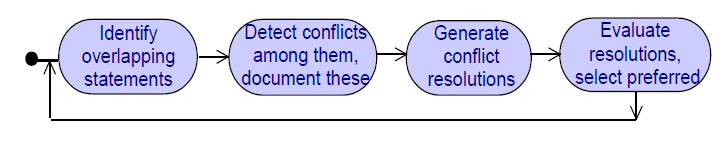
\includegraphics[width=0.5\textwidth]{img/requirements/conflicts.png}
      \caption{Managing conflicts}
      \label{fig:conflicts}
\end{figure}
Analizzando nel dettaglio la figura \ref{fig:conflicts} abbiamo:
\begin{enumerate}
      \item Nella fase di sovrapposizione/overlap indichiamo il riferimento a
            termini o fenomeni comuni e sono le precondizioni del conflitto.
      \item La fase di riconoscimento può essere fatta informalmente, tramite
            euristiche sulle categorie dei requisiti in conflitto, o formalmente. Il
            riconoscimento deve essere documentato per una successiva risoluzione e analisi
            dell'impatto. Si usano strumenti come l'interaction matrix che presenta su
            righe e colonne gli statement e negli incroci indica:
            \begin{equation}
                  M[s_i,s_j] = \begin{cases}
                        1    & \text{ conflitto}                  \\
                        0    & \text{ nessun overlap}             \\
                        1000 & \text{ overlap ma senza conflitto} \\
                  \end{cases}
            \end{equation}
            Avendo, per ogni statement $S_i$, indicando con $S_i$ la riga/colonna
            corrispondente (sono uguali):
            \begin{equation}
                  conflicts(S_i) = \left(\sum_{s \ \in \ S_i} s \right) \mod 1000
            \end{equation}
            \begin{equation}
                  nonConflictingOverlaps(S_i) = \left\lfloor \sum_{s \ \in \ S_i} s / 1000 \right\rfloor
            \end{equation}
      \item La terza fase è strutturata nel seguente modo:
            \begin{itemize}
                  \item Esplorare prima più risoluzioni, generate tramite tecniche
                        di elicitation e usando tattiche di risoluzione dei conflitti:
                        \begin{itemize}
                              \item Evitare condizioni a contorno
                              \item Ripristinare statement in conflitto
                              \item Indebolire gli statement in conflitto
                              \item Non considerare statement a bassa priorità
                              \item Approfondire source e target del conflitto
                        \end{itemize}
                  \item Confrontare, selezionare e concordare il preferito poi.
            \end{itemize}
            Si trasformano quindi statement in conflitto (e parti coinvolte) in nuovi requisiti.
      \item Nella quarta fase si usano vari criteri per la scelta:
            \begin{itemize}
                  \item Contributo a requisiti non funzionali critici.
                  \item Contributo alla risoluzione di altri conflitti e rischi.
                  \item Applicazione dei principi di risk analysis.
            \end{itemize}
\end{enumerate}

La parte di \textbf{Requirements prioritization} consiste nel fornire ai vari
requisti una prioritizzazione, per vari scopi:
\begin{itemize}
      \item Risoluzione dei conflitti.
      \item Limitazioni delle risorse.
      \item Sviluppo incrementale.
      \item Ri-pianificazione a causa di problemi imprevisti.
\end{itemize}
e si hanno vari principi per una buona riuscita della stessa, che può essere
svolta tramite:
\begin{enumerate}
      \item \textbf{Livelli ordinati} di uguale priorità, in un piccolo numero.
      \item \textbf{Livelli relativi} come ad esempio \textit{maggiore di}.
      \item \textbf{Requisiti comparabili}: stessa granularità, stesso livello di
            astrazione.
      \item \textbf{Requisiti non mutuamente dipendenti}.
      \item Un \textbf{accordo} con i vari partecipanti e stakeholder.
\end{enumerate}
Per i primi 3 prinicpi si può utilizzare il metodo \textbf{Value-cost	prioritization}:
\begin{itemize}
      \item stimare il contributo relativo di ogni requisito all'interno del
            \textbf{valore} del progetto
      \item stimare il contributo relativo di ogni requisito all'interno del
            \textbf{costo} del progetto
      \item si rappresenta il diagramma valore-costo (fig \ref{fig:cost-value-diagram})
\end{itemize}

\begin{figure}[!ht]
      \centering
      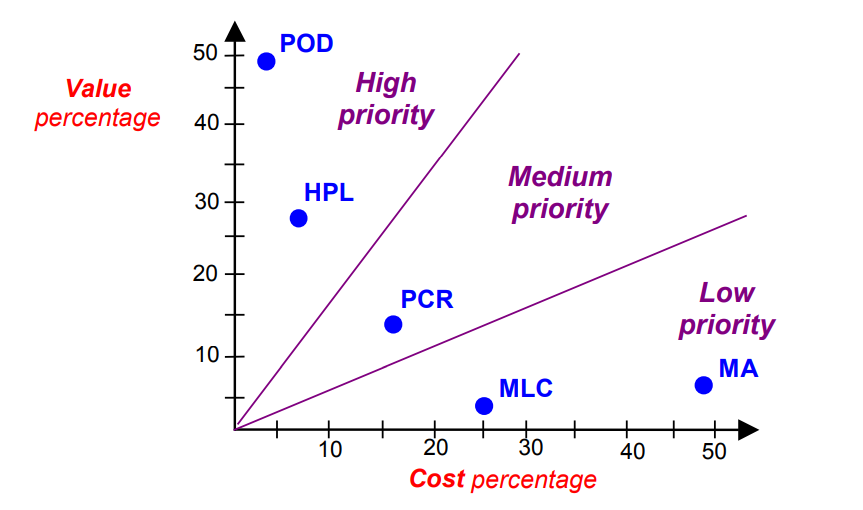
\includegraphics[width=0.5\textwidth]{img/requirements/cost-value-diagram.png}
      \caption{Diagramma Cost-value}
      \label{fig:cost-value-diagram}
\end{figure}

Si usa quindi la tecnica AHP dalla Decision Theory dove si cerca di capire in che
proporzione ogni requisito $R_i$ contribuisce al criterio $crit$, che sarà prima
il valore, $crit = value$, e poi il costo, $crit = cost$. Si hanno quindi due step:
\begin{enumerate}
      \item Si usa la comparison matrix stimando i contributi di ogni requisito sul
            criterio da studiare. Avendo $N$ requisiti:
            \begin{equation}
                  R_{i, j} = \frac{1}{R_{i, j}}, \ \ \ \text{se} \ 1 \leq i, j\leq N
            \end{equation}
            Dalla comparison matrix si hanno dei valori, più basso è il valore di $R_{ij}$
            allora $R_i$ contribuisce equamente insieme a $R_j$, più è alto il valore allora
            $R_i$ contribuisce  di molto più rispetto a $R_j$
      \item Si determina quanto questo si distribuisce tra tutti i requisti, tramite
            gli autovalori della matrice. Inoltre le colonne vengono normalizzate tramite:
            \begin{equation}
                  R_{i, j} = \frac{R_{i, j}}{\sum_i R_{i, j}}
            \end{equation}
            e aggiungendo la media sulle righe per valutare il contributo del requisito
            sul criterio.
\end{enumerate}
AHP permette di assicurare stime e rapporti consistenti.

\subsection{Specification \& documentation}
In questa fase si documentano in modo preciso i requisiti scoperti. Si descrivono
in modo preciso le feature e i concetti rilevanti per il progetto. Nel dettaglio
si definiscono in modo preciso:
\begin{itemize}
      \item Obiettivi, concetti, proprietà di dominio rilevanti, requisiti di
            sistema/software, ipotesi, responsabilità
      \item La motivazione delle opzioni scelte
      \item Un'indicazione sulle varianti e sulle evoluzioni previste
\end{itemize}

Il documento deve avere una struttura coerente. Tale documento è detto
\textbf{Requirements Document} (RD). Qualora i requisti siano stati messi online
si procede alla costruzione di un database che tiene traccia dei requisti. In ogni
caso il contenuto deve essere accessibile e comprensibile da tutte le parti
interessate, aggiungendo spesso in allegato anche costi, workplan e piani di delivery.
Bisogna capire come effettivamente documentare i requisiti.

\subsubsection{Non-formal notation}
La prima opzione è l'utilizzo del linguaggio naturale in modo svincolato. Si ha
una forte espressività ma, in assenza di regole sulla scrittura si rischia di
produrre una sorta di romanzo, producendo qualcosa di poco gestibile. Il linguaggio
naturale inoltre può nascondere ambiguità. Usando il linguaggio naturale privo
di vincoli si hanno quindi rischi ma si può usare un linguaggio naturale strutturato,
per ottenere tale linguaggio si introducono quindi due tipi di regole:
\begin{enumerate}
      \item \textbf{Local rules}, che riguardano la scrittura del singolo requisito.
      \item \textbf{Global rules}, che riguardano le regole sulla scrittura
            dell'intero documento e sull'insieme dei requisti.
\end{enumerate}
Abbiamo però alcune regole stilistiche generali:
\begin{itemize}
      \item Scrivere pensando a chi deve leggere, che deve essere ben identificato.
      \item Spiegare cosa stiamo per scrivere prima di specificarlo nel dettaglio.
      \item Prima motivare le scelte, indicare le scelte e poi fare un sommario delle stesse.
      \item Assicurarsi che ogni concetto usato nei requisiti sia stato prima ben definito.
      \item Chiedersi se quanto scritto è comprensibile e rilevante.
      \item Per ogni frase/elemento del documento indicare uno e un solo requisito
            o assunzione o proprietà di dominio, evitando di mischiare troppe cose.
      \item Scrivere frasi brevi.
      \item Distinguere ciò che è obbligatorio da ciò che è desiderabile.
      \item Evitare acronimi non necessari ed evitare l'abuso del gergo informatico.
      \item Usare esempi esplicativi.
      \item Usare diagrammi o illustrazioni quando utile.
\end{itemize}

In termini di \textit{local rules} si hanno dei template per scrivere i requisiti,
usando anche un solo standard per tutti i requisti. Un esempio di template potrebbe contenere:
\begin{itemize}
      \item Identificatore del requisito, con uno schema di naming significativo.
      \item Categoria del requisito (funzionale, assunzione $\dots$).
      \item Specifica del requisito (usando le regole stilistiche).
      \item Criterio di fit o test di accettazione, il quale è usato quindi per
            quantità/concetti misurabili, essendo critico quindi per requisiti non funzionali.
      \item Fonti di elicitazione.
      \item Motivazioni.
      \item Interazioni con altri requisti (contribuzioni, dipendenze e conflitti).
      \item Livello di priorità.
      \item Livelli di stabilità (per indicare le chance di cambiamenti).
\end{itemize}
Per le \textit{global rules} si ha una forma standard data da IEEE std-830, il
più diffuso. Si hanno varie macro-categorie a loro volta suddivise in:
\begin{enumerate}
      \item \textit{Introduzione}: si specifica anche quale parte del documento
            interessi ai vari stakeholder:
            \begin{enumerate}
                  \item Motivazioni del documento.
                  \item Scopo del prodotto.
                  \item Definizioni, acronimi, sigle e abbreviazioni.
                  \item Reference, fonti di elicitazione.
                  \item Overview dell'organizzazione del documento.
            \end{enumerate}
      \item \textit{Descrizione generale}
            \begin{enumerate}
                  \item Prospettive del prodotto.
                  \item Funzionalità principali.
                  \item Caratterizzazione degli utenti.
                  \item Vincoli generali sull'ambiente (che non possono esse modificati
                        ma con i quali si deve integrare il prodotto).
                  \item Assunzioni sul prodotto e dipendenze del prodotto.
                  \item Ripartizione dei requisti.
            \end{enumerate}
      \item \textit{Requisiti specifici} usando magari il template visto prima. Si
            hanno quindi varie categorie di requisiti che articolano le varie sezioni del capitolo:
            \begin{enumerate}
                  \item Requisiti funzionali, che a sua volta può avere un'organizzazione
                        interna in base a vari fattori.
                  \item Requisiti per l'interfaccia esterna.
                  \item Requisiti per le prestazioni.
                  \item Vincoli di progettazione.
                  \item Attributi di qualità del software
                  \item Altri requisiti
            \end{enumerate}
      \item Appendice.
      \item Indice.
\end{enumerate}

Una variante per il template VOLERE dove si hanno sezioni esplicite per proprietà
del dominio, costi, rischi, piano di lavoro di sviluppo etc$\dots$

Il RD può essere dislocato in diversi posti, per esempio: la sezione della
descrizione generale può essere messa sul repository, mentre la sezione dei
requisiti specifici potrebbe essere su Trello.

\subsubsection{Semi-formal notation}
Si hanno anche opzioni aggiuntive oltre al linguaggio naturale. Una prima alternativa
sono i diagrammi, dove si ha una notazione semi-formale, in quanto si ha una sintassi
formale essendo i vari diagrammi formalmente definiti ma l'interpretazione degli
stessi può comunque essere ambigua.

I diagrammi sono utili per complementare quanto scritto in linguaggio naturale, che
spesso risulta troppo complesso e articolato. Un diagramma può semplificare quanto
scritto e rappresentare il tutto in modo compatto. L'uso di diagrammi permette
di ottenere un metodo di comunicazione più semplicemente e viene usato per aspetti
specifici del sistema. Si ha comunque la stessa ambiguità di interpretazione
che si aveva nei linguaggi naturali.

I diagrammi sono tra loro complementari ma hanno anche delle intersezioni tra
loro e anche con il testo e tutto deve comunque restare coerente. Si rischia di
introdurre inconsistenze.

Si hanno alcune regole di consistenza per i diagrammi che vengono usate da diversi
strumenti per verificare la consistenza tra i vari diagrammi.

A questo punto è doveroso citare uno degli standard per la modellazione di
diagrammi: \textbf{Unified Modeling Languag}e (UML). Al suo interno si hanno, con
regole di coerenza tra essi:
\begin{itemize}
      \item class diagrams
      \item use case diagrams
      \item sequence diagrams
      \item state diagrams
\end{itemize}

In conclusione i diagrammi hanno il pro di essere in grado di dare una buona panoramica
e struttura/comportamento, facile da trasmettere e comprendere, di aspetti importanti.
Sono inoltre supportati da vari tool di analisi.

Il contro è sempre la specifica ambigua semi-formale che può anche limitare l'analisi
degli stessi. Inoltre si concentrano solo su aspetti funzionali e strutturali.

Si hanno anche gli statechart per la descrizione di sistemi paralleli che usano
la semantica interleaving ovvero per 2 transizioni che si attivano nello stesso
stato, una viene presa dopo l'altra, in modo non deterministico.
\paragraph{Problem diagram (context diagram)}
Un primo esempio di digramma utilizzato è il \textbf{problem diagram}
\ref{fig:problemDiagram}, il quale
descrive i requisiti a livello di sistema.

In questo diagramma si descrive il problema che si vuole risolvere, mostrando le
componenti del sistema e le loro interazioni. Si può specificare testualmente un
requisito e riferirlo alle componenti del sistema citate nel requisito, che è
posto in un ellisse tratteggiato. Posso avere riferimenti e vincoli sulle
componenti a partire dal requisito. Tutte le interazioni sono decorate con gli
eventi che sono rilevanti per l'interazione con il produttore dell'evento indicato
tramite le maiuscole e il nome dell'evento, a loro volta separati da “!”.

Ogni componente del sistema è indicata tramite un rettangolo in cui è presente
una doppia linea a sinistra. Il sistema comunica con diversi elementi dell'ambiente,
indicati da rettangoli.

Con questo tipo di diagramma si cattura il contesto del requisito, legandolo
componenti dell'ambiente e componenti del sistema, tramite specifici eventi.
Si identificano a colpo d'occhio gli elementi rilevanti per un certo requisito.
\begin{figure}[!ht]
      \centering
      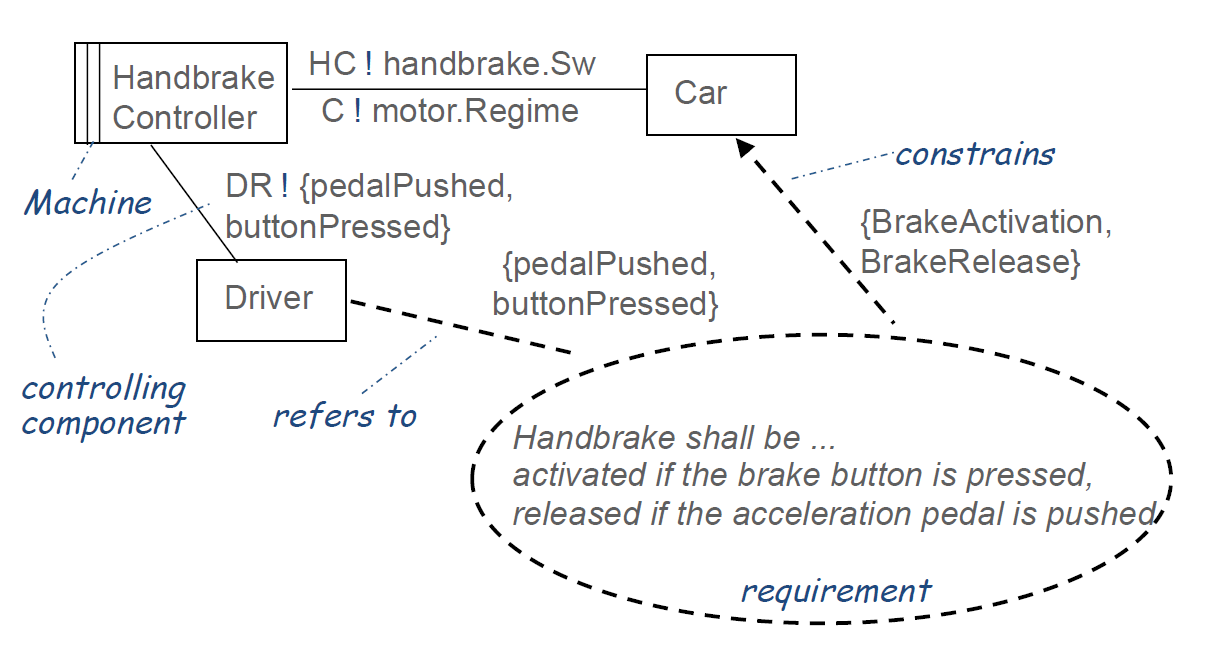
\includegraphics[width = \textwidth]{img/requirements/PD.png}
      \caption{Esempio di Problem Diagram}
      \label{fig:problemDiagram}
\end{figure}

Questa rappresentazione può prendere la forma di veri e propri pattern detti
\textbf{problem pattern} per semplificare la rappresentazione. Si ottengono i
\textbf{frame diagrams} (fig \ref{fig:frame-diagram}), che hanno la stessa
rappresentazione dei problem diagram con la differenza che si ha qualche informazione in più:
\begin{itemize}
      \item \textbf{Tipo di componente}, indicato con un quadratino in basso a
            destra nel rettangolo della componente, specificato da una lettera:
            \begin{itemize}
                  \item C: causal, causa-effetto
                  \item B: biddable, non predicibile
                  \item X: lexical, lessicale, specifica artefatti
            \end{itemize}
      \item \textbf{Tipo di evento} (posto) dopo il “!” sopra descritto, specificato
            da una lettera:
            \begin{itemize}
                  \item C: causal, diretta conseguenza di altri eventi
                  \item E: event, che non sono diretta conseguenza ma che sono prodotti
                        in modo spontaneo
                  \item X: lexical, dati che vengono utilizzati per produrre qualcosa
            \end{itemize}
\end{itemize}
Tali pattern vengono istanziati nei vari casi specifici.

\begin{figure}[!ht]
      \centering
      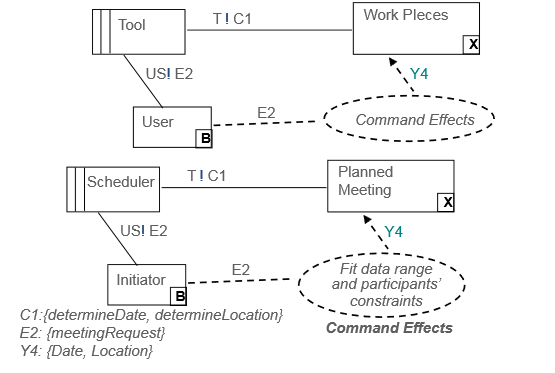
\includegraphics[width = \textwidth]{img/requirements/frame-diagram.png}
      \caption{Esempio di Frame Diagram}
      \label{fig:frame-diagram}
\end{figure}
\paragraph{Diagrammi ER}
Un altro diagramma tipico è quello ER per specificare entità che entrano in gioco
in certi aspetti dei requisiti, specificandole in modo schematico. Si usano anche
diagrammi di dominio, di classe etc$\dots$, non descrivendo più comportamenti
ma strutture, domini etc$\dots$
\paragraph{Diagrammi SADT}
I \textbf{SADT diagrams} permettono di specificare il comportamento di alcune
attività scomponendolo e aggiungendo varie informazioni. Possiamo avere due tipi
di diagrammi:
\begin{enumerate}
      \item \textbf{Actigram} \ref{fig:actigram}: sono di tipo \textit{activity-driven}
            e si concentrano sulle attività e sul mostrare le dipendenze tra le attività
            in termini di dati. Le attività sono indicate dentro rettangoli e si hanno
            una serie di frecce che a seconda della direzione variano il significato:
            \begin{itemize}
                  \item $\to$ (in entrata all'attività) per l'input di dati.
                  \item $\to$ (in uscita dall'attività) per l'output di dati.
                  \item $\downarrow$ per il data/event controlling, ovvero dati o
                        eventi che controllano il comportamento dell'attività, sono magari
                        aspetti di configurazione etc$\dots$ che influenzano l'attività
                  \item $\uparrow$ per l'unità che processerà l'attività, questa può
                        essere opzionale.
            \end{itemize}
            \begin{figure}[!ht]
                  \centering
                  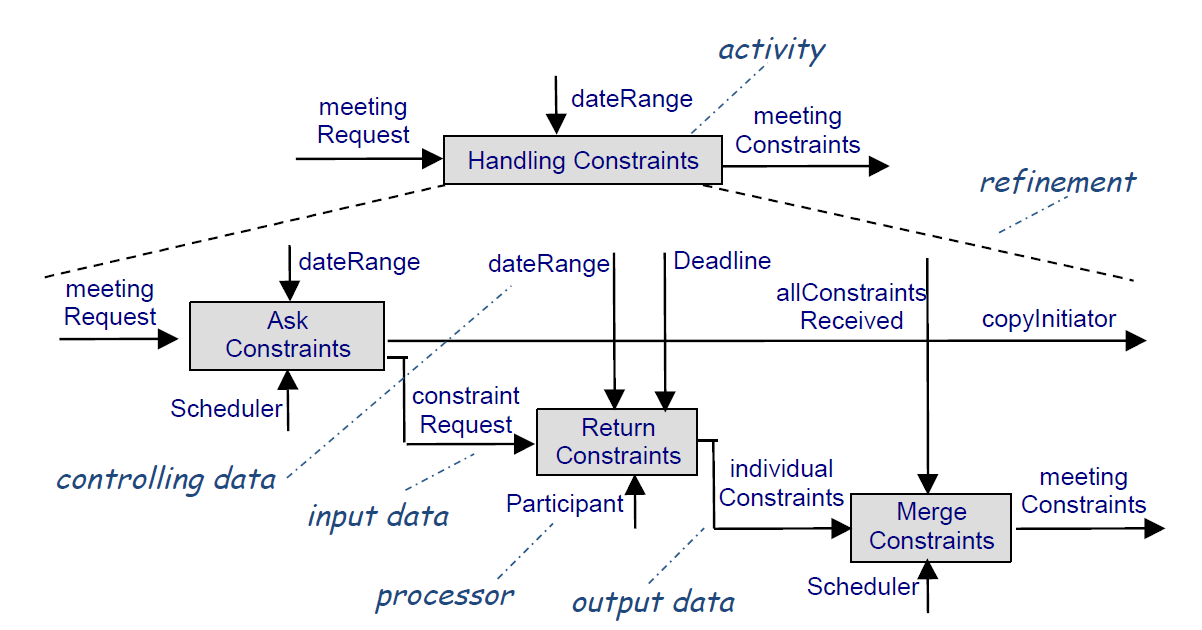
\includegraphics[width = \textwidth]{img/requirements/actigram.png}
                  \caption{Actigram}
                  \label{fig:actigram}
            \end{figure}
      \item \textbf{Datagram} \ref{fig:datagram}: sono di tipo \textit{data-driven},
            si concentrano sui dati e mostrano le dipendenze tra i dati in termini di
            attività. I dati sono indicate dentro rettangoli e si hanno una serie di frecce
            che a seconda della direzione variano il significato:
            \begin{itemize}
                  \item $\to$ (in entrata al dato) per l'input di attività che producono il dato.
                  \item $\to$ (in uscita daal dato) per l'output di attività verso le quali serve il dato.
                  \item $\downarrow$ per le attività di validazione del dato.
                  \item $\uparrow$ per le risorse necessarie a memorizzare e gestire il dato.
            \end{itemize}
            \begin{figure}[!ht]
                  \centering
                  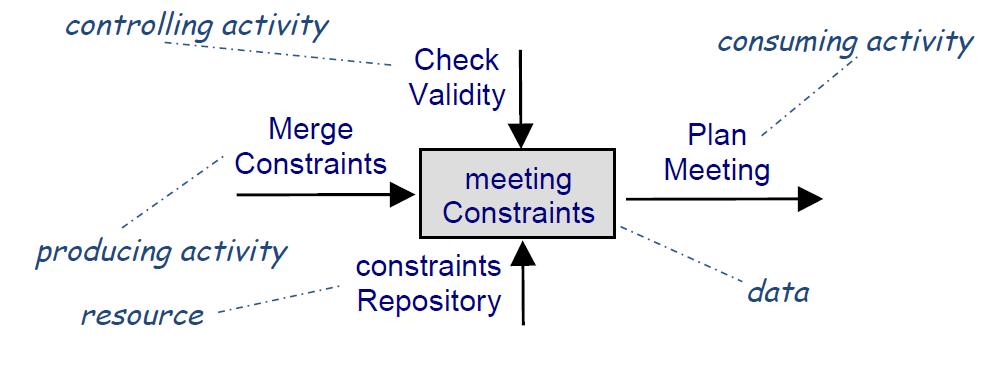
\includegraphics[width=\textwidth]{img/requirements/datagram.png}
                  \caption{Datagram}
                  \label{fig:datagram}
            \end{figure}
\end{enumerate}
La coerenza tra di due diagrammi è fondamentale avendo una rapporto di dualità
tra essi quindi i dati e le attività presenti in uno devono apparire anche nell'altro.

Questo strumento si prestano a documentare workflow molto semplici. In ogni caso:
\begin{itemize}
      \item Ogni attività deve avere un input e un output.
      \item Tutti i dati devono avere un produttore e un consumatore.
      \item I dati I/O di un'attività devono apparire come dati I/O delle sotto-attività.
      \item Ogni attività in un datagramm deve essere definita in un actigramma.
\end{itemize}
\paragraph{Dataflow diagram}
I \textbf{Dataflow diagram} \ref{fig:dataflow-diagram} cattura tutte le operazioni
di sistema collegate dalla dipendenza dei dati,
corrisponde ad un actigram più semplice ma meno espressivo. Si definiscono:
\begin{itemize}
      \item \textbf{ovali}: per i componenti
      \item \textbf{frecce}: specificano i flussi dei dati
\end{itemize}

\begin{figure}[!ht]
      \centering
      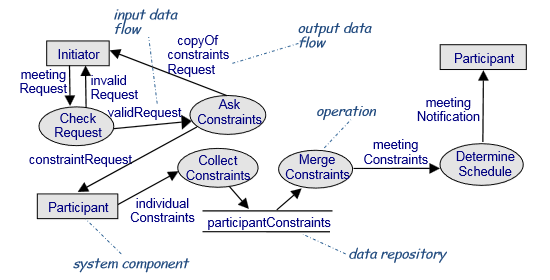
\includegraphics[width=\textwidth]{img/requirements/dataflow-diagram.png}
      \caption{Dataflow diagram}
      \label{fig:dataflow-diagram}
\end{figure}

\paragraph{Use case Diagram}
Un altro diagramma classico è lo \textbf{use case diagram} per visualizzare i
requisiti identificati, che prendono forma di casi d'uso con gli attori che partecipano
allo svolgimento dei requisiti.
\paragraph{Event trace diagrams}
Un altro strumento utile nella definizione di workflow è l'\textbf{event trace diagrams}
\ref{fig:etd}, ovvero i diagrammi di sequenza. Se ne hanno vari tipi con sintassi
più o meno ricche ma in generale si hanno $N$ elementi che partecipano all'esecuzione
che viene mostrata visualmente tramite richieste e risposte, sincrone o meno,
che vengono indicate cronologicamente dall'alto al basso.
\begin{figure}[!ht]
      \centering
      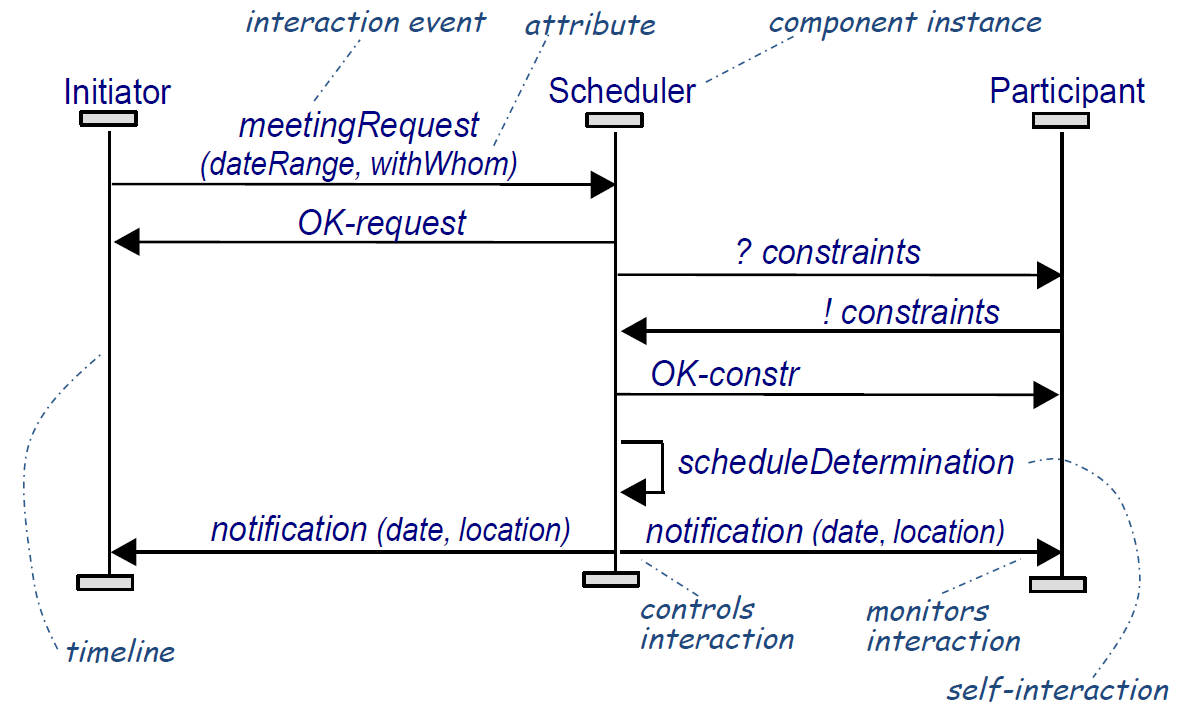
\includegraphics[width=\textwidth]{img/requirements/etd.png}
      \caption{Event trace diagrams}
      \label{fig:etd}
\end{figure}
Questa visualizzazione compatta aiuta nel momento in cui il linguaggio naturale
diventa troppo complesso e verboso per spiegare una certa sequenza di azioni.
\paragraph{State machine diagram}
Un altro diagramma usato è lo \textbf{state machine diagram} \ref{fig:smd} per
mostrare in quali stati un particolare elemento si trova e quali transizioni/eventi
modificano i suoi stati. Questi diagrammi sono utili in quanto in modo compatto
rappresentano il ciclo di vita di una certa componente, facilitando la creazione
del sistema.
\begin{figure}[!ht]
      \centering
      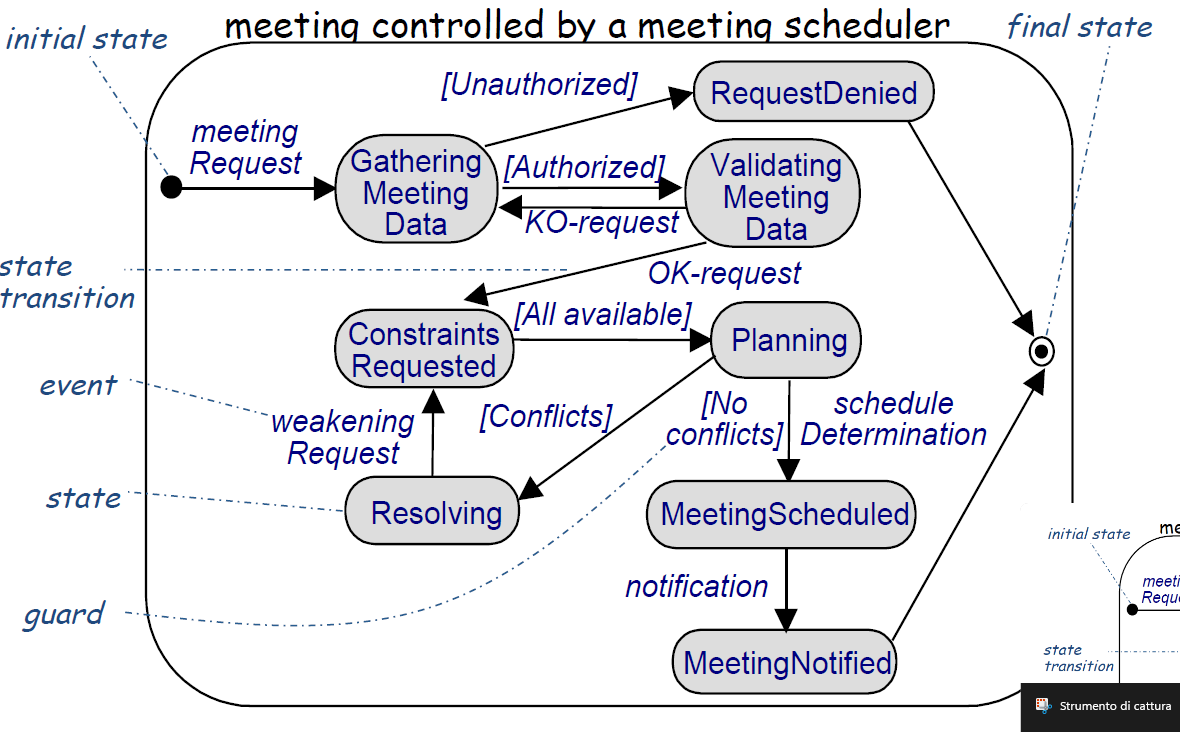
\includegraphics[width=\textwidth]{img/requirements/smd.png}
      \caption{State machine diagram}
      \label{fig:smd}
\end{figure}
\paragraph{R-net diagram}
Come altro diagramma abbiamo il \textbf{R-net diagram} \ref{fig:r-net-diagram} che permette di mostrare
come reagisce un sistema in base ad un certo stimolo. È quindi un albero che parte
con uno stimolo, dopo il begin, posto in un esagono e si sviluppo in base alle
varie alternative in corrispondenza di punti di decisione (indicati come pallini).
Nei rettangoli si hanno le azioni che sono svolte in conseguenza allo stimolo.
\begin{figure}[!ht]
      \centering
      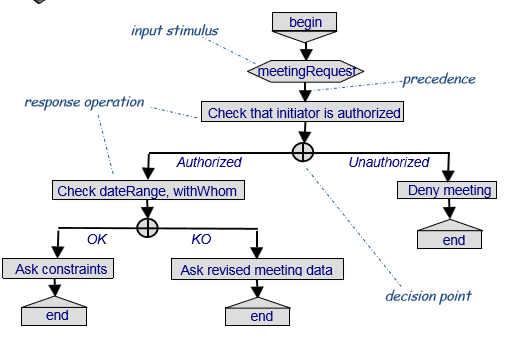
\includegraphics[width=\textwidth]{img/requirements/r-net-diagram.png}
      \caption{R-net diagram}
      \label{fig:r-net-diagram}
\end{figure}
\subsection{Formal notation}
Si ha quindi in generale la necessità di una semantica formale per aspetti
mission - critical e la cosa non viene garantita dai diagrammi ma si hanno linguaggi
apposta (e diagrammi apposta) la cui creazione/gestione/documentazione è assai
costosa per cui vengono usati solo in casi estremamente specifici. Approfondiamo
quindi questi linguaggi e questa notazione.

Si parla sia di sintassi che di semantica. Tali definizioni formali permettono
che il compilatore sia in grado di processare tali specifiche. Si ha quindi un
livello di precisione alto e non si ha ambiguità, permettendo analisi di consistenza
e coerenza delle specifiche.

Una sintassi/semantica formale è quella data dalla logica proposizionale e dalle
formule ben formate. Si ha quindi un linguaggio basato sui connettori logici e
sulle regole per avere formule ben formate.

Ogni statement può quindi essere interpretato con il valore di verità con le
regole definite dalla logica e dalle tabelle di verità. Si vede quanto produrre
tutto questo per un progetto enorme risulti costoso. Vengono quindi usate le
classiche regole di inferenza. Si usa anche la logica predicativa del primo ordine.

Un altro strumento usato è la logica temporale con l'aggiunta dei connettivi temporali.

Si ha un approccio formale anche su specifiche state-based dove si specifica in
modo formale cosa sia l'insieme degli stati che il sistema può attraversare e
come delle operazioni modificano lo stato.

Si usano linguaggi come $Z$ basati sulla teoria degli insiemi. Ogni stato è
caratterizzato da pre e post condizioni e si studiano le regole in termini di
invarianti che lo stato deve soddisfare.

Con Z si producono schemi dove si specifica un certo elemento, gli attributi di
stato con P che indica l'insieme delle parti che precede il tipo. Si ha poi un
invariante per gli attributi che definisce l'elemento. Si ha quindi una caratterizzazione
basata sulla teoria degli insiemi. Si hanno sia tipi primitivi che strutturati.
Per definire invece le modifiche che portano a nuovi stati.

Sopra si hanno tutti gli elementi coinvolti nell'operazione. La prima linea della
parte sotto è per le precondizioni, quella sotto per le postcondizioni, entrambe
con la notazione insiemistica. Gli elementi sono inoltre così decorati:
\begin{itemize}
      \item stateVar?:Type indica una variabile di input
      \item stateVar':Type indica una variabile di output mutevoli
      \item stateVar!:Type indica una variabile di output esterne e non mutevoli
      \item $\Delta$ schema indica che si ha una modifica delle variabili importate
            dallo schema
      \item $\Xi$ schema indica che non si ha una modifica delle variabili importate
            dallo schema
\end{itemize}

Il cambiamento di stati ben definito diventa studiabile e simulabile, studiando
lo spazio di comportamenti del sistema a questo livello di astrazione, individuando
problemi che porterebbero alla correzione di requisiti. Si può avere anche
l'inclusione di più schemi. Con questa specifica state-based si hanno vari pro:
\begin{itemize}
      \item automazione semplice grazie a logica, matematica discreta, studio degli
            invarianti etc$\dots$
      \item ottimi meccanismi di strutturazione per comporre unità e strutture
            stati complessi
      \item permette l'analisi automatica: type checking, consistency checking,
            etc$\dots$
\end{itemize}

Di contro non permette di studiare altro se non aspetti funzionali e non ha
un'historical referencing.

Si ha anche una specifica algebrica per formalizzare le leggi che compongono le
operazioni, viste come funzioni matematiche senza esplicita nozione di stato.
Si ha invece un system history avendo una “traccia” delle operazioni.

Si hanno tipi di dato astratti, parametrizzazione, equazioni condizionali e funzioni
parziali. Si hanno tre tipi di operazione:
\begin{enumerate}
      \item modifiers, per produrre qualsiasi istanza di concetto mediante composizione
            con altri modifier
      \item generators, ovvero un sottoinsieme minimo di modifiers per generare
            qualsiasi istanza di concetto con un numero minimo di composizioni
      \item obsevers, per ottenere informazioni pertinenti su qualsiasi istanza di
            concetto
\end{enumerate}

Spesso si hanno funzioni ricorsive.

Come vantaggi si hanno:
\begin{itemize}
      \item analisi automatica efficiente
      \item specifiche eseguibili
      \item ricchi meccanismi di strutturazione (import, ereditarietà $\dots$)
\end{itemize}

Di contro si ha una limitata potenza espressiva (solo equazioni senza historical
referencing) e una forte vicinanza alla programmazione (comportando difficoltà
di validazione in caso, ad esempio, di ricorsioni).

Tendenzialmente i limiti della notazione formale sono sempre questi (oltre alla
difficoltà di lettura/scrittura), anche se permette alta precisione, pochi difetti
di specifica, analisi sofisticata (anche automatica), generazione di artefatti
come test cases, codice etc$\dots$.

Ricapitolando:
\begin{itemize}
      \item il linguaggio naturale “puro” non è un'opzione
      \item il linguaggio naturale strutturato è quello più usato
      \item i diagrammi sono un'ottima aggiunta al linguaggio naturale
      \item la notazione formale è usata in rare circostanze
\end{itemize}
\subsection{Validation \& verification}
Siamo quindi all'ultima delle quattro fasi, dove bisogna validare i requisiti.
Si hanno vari approcci per validare la qualità dei requisiti:
\begin{itemize}
      \item \textbf{Analisi e revisione dei singoli requisiti}: è manuale e costoso in
            termini di tempo ma si può sempre fare
      \item \textbf{Interrogare il database delle specifiche}: è automatico ma non
            controlla la qualità di tutti
      \item \textbf{Usare le specification animation}: servono dei requisiti eseguibili,
            buono per trovare dei bug
      \item \textbf{Check formale}: richiede requisiti specificati in modo
            formale e può rivelare tutti i bug.
\end{itemize}

\subsubsection{Analisi e revisione dei singoli requisiti}
Questo è sempre applicabile ma va fatto manualmente impiegando molto tempo. La
prima operazione consiste nel ricercare errori nel Requirements Document. Spesso
questi sono gli errori più numerosi e pericolosi e possono avere varia natura:
\begin{itemize}
      \item Omissione
      \item Contraddizione
      \item Inadeguatezza
      \item Ambiguità
      \item Incommensurabilità
      \item Rumore
      \item Eccesso di specificità
      \item Scarsa struttura
      \item Opacità
\end{itemize}
Bisogna quindi individuare quanti più problemi possibili nel Requirements Document,
validarli (vedendo se le informazioni utili sono necessarie), verificarli (vedendo
se sono completi e consistenti) e confermare non ambiguità, misurabilità,
fattibilità, buona struttura, etc$\dots$

Bisogna quindi fare il report dei problemi, analizzarne la causa e correggerli.
Questa operazione viene fatta selezionando personale che ispeziona il Requirements
Document individualmente per poi confrontare le opinioni. Tali persone possono
essere interne ai project members o recensori esterni. Questo viene spesso fatto
anche per il codice sorgente e quindi si è mostrato che è empiricamente utile
anche per le revisioni del Requirements Document.

La revisione può essere effettuata in vari modi:
\begin{itemize}
      \item \textbf{Free mode}: senza direttiva su cosa cercare e dove.
      \item \textbf{Checklist-based}: indicando una lista di cose da controllare.
      \item \textbf{Process-based}: dove si hanno ruoli specifici, procedure dettagliate,
            tecniche di analisi etc$\dots$, rendendo questa la modalità più efficace.
\end{itemize}
Il report deve essere fatto in modo informativo e accurato, senza opinioni o
commenti offensivi (anche se può essere lasciato uno spazio per i commenti liberi).
Ovviamente le revisione deve essere fatta possibilmente da personale diverso da
quello che scrive il Requirements Document e tale personale deve rappresentare
tutti gli stakeholder con le varie conoscenze pregresse.

A livelli di tempo il controllo deve essere effettuato ne troppo presto ne troppo
tardi ma con incontri ripetuti per ottenere la massima efficacia.

Ci si deve inoltre concentrare sulle parti più critiche, che devono essere meglio
analizzate. Dal punto di vista delle checklist se ne hanno diverse:
\begin{itemize}
      \item \textbf{Defect-driven}: lista dei difetti tipici, strutturate tramite
            un elenco di domande generiche.
      \item \textbf{Quality-specific}: lista più specializzata di quella defect-driven,
            specializzandosi su requisiti non funzionali.
      \item \textbf{Domain-specific}: lista specializzata nei concetti e nelle
            operazioni di dominio per aiutare nella ricerca dei difetti:
      \item \textbf{language-based}: lista specializzata nei costrutti legati ai linguaggi.
            In questa parte si analizzano anche i diagrammi, si analizzando anche
            linguaggi di specifica come Z.
\end{itemize}
Si usano anche delle \textbf{checking decision tables} che hanno in input $N$
condizioni booleane ($\{T, F\}$) e una serie di eventi che si hanno in conseguenza
allo stato delle condizioni, specificando se accadono o meno. Si ha che se il
numero di combinazione dei vari casi specificati dalle condizioni in input è minore
$2^N$ (se ho meno colonne del dovuto nella tabella di verità) allora mancano dei
casi da analizzare mentre se è maggiore si hanno dei casi ridondanti.

Questo tipo di analisi è quindi applicabile potenzialmente alla ricerca di ogni
difetto (anche se non si ha garanzia di riconoscerli tutti, per quanto critici,
anche se con un mix delle tecniche spiegate si raggiungono ottimi risultati).
I costi restano elevati sia in termini monetari che di tempo.
\subsubsection{Interrogare il database delle specifiche}
Questo, a livello superficiale, può essere fatto in modo automatico ma è appunto
un check parziale. Questa tecnica è specifica per casi particolari, dove le
specifiche sono memorizzate in un database. Le query acquisiscono controlli per
la coerenza strutturale intra o inter-diagrammi e tali query possono essere generate
a partire dall'ER. Si parla anche di press-button mode quando si ha una lista
di query prescritte per la violazione delle regole di coerenza standard.
\subsubsection{Usare le specification animation}
Sono ottime per i non esperti per identificare i problemi ma sono limitate alle
specifiche “eseguibili”, consentendo quindi solo un check parziale. Si vuole
verificare l'adeguatezza dei requisiti rispetto alle effettive necessità. Si
hanno due approcci tipici:
\begin{enumerate}
      \item Mostrare una vera interazione cono lo scenario. In questo caso gli
            strumenti di “promulgazione” possono essere utilizzati sul diagramma NET ma
            ovviamente si ha il problema del range di copertura dei problemi dato dallo
            scenario.
      \item Usare tool per l'animazione delle specifiche. Si procedere generando
            un modello eseguibile e si procede alla simulazione (provvedendo a stimoli e
            vedendo il risultato) per poi raccogliere il feedback dell'utente. Si può avere:
            \begin{itemize}
                  \item Formato testuale, con comandi di input e poi esecuzione.
                  \item Formato a diagrammi, con un input che comporta l'evoluzione
                        di parti del diagramma.
                  \item Scena vera e propria con pannelli per l'input e scene animate
                        nell'ambiente scelto.
            \end{itemize}
\end{enumerate}
In ogni caso si ha un approccio model-based, si parla infatti di model-driven
development (sviluppando fin dall'inizio modellando il comportamento del software),
e si hanno vari tool per i vari linguaggi di specifica (SCR, LTSA etc$\dots$).

Tra i pro si hanno:
\begin{itemize}
      \item È modo migliore per verificare l'adeguatezza rispetto ai bisogni reali,
            all'ambiente reale
      \item Permette la facile interazione con gli stakeholder secondo la filosofia
            WYSIWYC (What You See Is What You Check)
      \item Estendibile per animare controesempi generati da altri strumenti.
      \item Le animazioni possono essere riusate per altri scenari.
\end{itemize}
Si hanno anche contro:
\begin{itemize}
      \item Si richiede un'attenta progettazione degli scenari che possono presentare
            problemi e non si ha garanzia di non trascurare problemi critici.
      \item Necessita specifiche formali.
\end{itemize}
\subsubsection{Check formale}
Questo permette di individuare un ottimo range di problemi ma richiede la notazione
formale, costosa, ed esperti. Si possono avere check sintattici per il linguaggio
(di specifica come Z) usato (syntax checking, type checking, static semantics
checking, le variabili utilizzate devono essere dichiarate e inizializzate,
devono essere utilizzate nello scope corretto etc$\dots$, circularity checking,
con il check delle postcondizioni etc$\dots$). Si può avere anche un check di
completezza e consistenza grazie al linguaggio e la verifica di proprietà:
\begin{itemize}
      \item Algoritmiche tramite model checking, per controllare se un modello di
            comportamento soddisfa un requisito, una proprietà di dominio o un presupposto,
            cercando violazione delle varie proprietà e generando eventuali controesempi
            o comunque specifiche della violazione (fattori utili nel debugging).
            Si possono controllare:
            \begin{itemize}
                  \item Raggiungibilità, tramite un grafo di raggiungibilità
                  \item Proprietà di safety, producendo controesempi
                  \item Proprietà di liveness, che comporta che una condizione potrebbe
                        non essere mai raggiunta in caso di risposta negativa del check
            \end{itemize}
            I pro del model checking sono:
            \begin{itemize}
                  \item Check completamente automatici
                  \item Ricerca esaustiva che porta a non tralasciare alcun difetto
                  \item L'uso di controesempi può rivelare errori sottili, difficili
                        da individuare altrimenti
                  \item È facile da abbinare agli animators per visualizzare le tracce
                  \item È sempre più usato per progetti mission critical
            \end{itemize}
            Ma si hanno anche dei contro:
            \begin{itemize}
                  \item Si rischia di avere un'esplosione combinatoria degli stati da
                        analizzare comportando l'impossibilità di essere eseguito per
                        sistemi molto grossi.
                  \item I controesempi possono essere complessi da capire e mostrano
                        solo i sintomi dei problemi, non le cause.
            \end{itemize}
      \item \textbf{Deduttive tramite theorem proving}. Il theorem proving viene
            usato per generare nuove specifiche tramite le regole di inferenza della logica.
            Si studiano le conseguenze logiche delle specifiche evidenziando eventuali
            inconsistenze in un processo generalmente iterativo per:
            \begin{itemize}
                  \item Fornire, accettare o rifiutare i lemmi.
                  \item Suggerire strategie di prova.
            \end{itemize}
            Si hanno diversi pro:
            \begin{itemize}
                  \item solidità e completezza del sistema formale utilizzato avendo
                        che ogni conclusione è corretta e che ogni conclusione corretta è derivabile
                  \item mostra specifiche incoerenti, conseguenze inadeguate
                  \item può essere usato per sistemi molto grandi, gestendo una gran
                        mole di dati tramite l'induzione
            \end{itemize}
            ma si hanno ovviamente dei contro:
            \begin{itemize}
                  \item è di uso difficile e richiede personale esperto
                  \item non produce controesempi
            \end{itemize}
\end{itemize}
Si hanno, per i check di consistenza quando servizi o comportamenti sono specificati
come relazioni I/O capendo:
\begin{itemize}
      \item se la relazione e una funzione (per isolare eventuali non determinismi)
      \item se la funzione è totale e quindi in grado di specificare ogni input
\end{itemize}
\subsection{Requirements changes}
I cambiamenti dei requisiti sono assai frequenti e quindi vanno gestiti. Si hanno
infatti varie iterazioni delle 4 fasi sopra descritte, formando la spirale.
In primis si hanno cambiamenti organizzativi, nuove normative, nuove opportunità,
tecnologie alternative, priorità e vincoli in evoluzione oltre ad una migliore
comprensione delle caratteristiche, dei punti di forza, dei limiti e dei difetti
del sistema. Un altro aspetto riguarda il problema di gestione delle informazioni,
in merito al mantenimento della coerenza, propagazione delle modifiche, controllo
delle versioni etc$\dots$

La gestione dei cambiamenti di requisito consiste quindi nel processo di anticipazione,
valutazione, accordo e propagazione dei cambiamenti nelle varie parti del
Requirements Document.

Innanzitutto bisogna identificare i cambiamenti probabili, valutare la probabilità
e documentarli al fine di:
\begin{itemize}
      \item Anticipare una risposta adeguata quando si verificherà il cambiamento,
            studiando eventuali dipendenze tra i requisiti.
      \item Progettare l'architettura che rimanga stabile nonostante i cambiamenti.
\end{itemize}
Inoltre, associando livelli di stabilità a gruppi di statement che definiscono le
varie feature. Si punta ad avere un numero di livelli comunque ridotto e di cercare
di permettere la comparabilità, che sia qualitativa e relativa.

Si usano regole euristiche per studiare i probabili cambiamenti, concentrandosi
sui requisiti che è più facile cambino, limitando così i costi. Il livello più
alto di stabilità viene definito per quelle feature presenti in ogni estensione/
variante del sistema. Si ha che aspetti intenzionali e concettuali, così come aspetti
funzionali e obiettivi chiave, sono più stabili di aspetti operazionali e non
funzionali (per esempio la comparsa di una notifica è più stabile del modo in cui
questa viene sviluppata$\dots$ importante è che ci sia la notifica).

La scelta tra varie alternative rende l'oggetto della scelta poco stabile anche
perché tale scelta può essere basata su una conoscenza incompleta, presupposti
volatili o generata da risoluzione di conflitti o contromisure a vari rischi.

Quindi tali requisiti sono poco stabili.

Un altro aspetto essenziale nello studio dell'evoluzione del progetto è legato
alla gestione della \textbf{tracciabilità} (detto anche \textbf{Traceability Management}
(TM)), che non è uno studio semplice nel caso dei requisiti ma torna comodo nel
momento dei loro cambiamenti per gestire il cambiamento dell'intero progetto. Si ha
che un certo aspetto è tracciabile se e solo se si sa perfettamente:
\begin{itemize}
      \item Da dove viene
      \item Perché esiste
      \item Per cosa sarà usato
      \item Come sarà usato
\end{itemize}
Possiamo quindi dire che il TM si occupa di identificare, documentare, recuperare
la logica e l'impatto degli elementi contenuti nel Requirements Document.

Si possono avere anche tracciamenti in merito o obiettivi specifici per determinati
requisiti, valutando l'impatto di eventuali modifiche e studiando come propagare
facilmente i cambiamenti per mantenere la coerenza ad altri elementi
dell'Requirements Document o, “scendendo di livello”, ad oggetti software.

Un aspetto centrale nel TM è rappresentato dai collegamenti di tracciabilità tra
gli elementi del Requirements Document. Tali collegamenti vanno scoperti,
memorizzati ed eventualmente recuperati. Tali collegamenti sono bidirezionali e,
ipotizzando uno schema verticale tra le varie fasi, si hanno:
\begin{itemize}
      \item \textbf{forward traceability}: Accessibilità dal source al target
            (che nello schema verticale sono le frecce verso il basso \ref{fig:traceability-diagram}).
            Il source motiva l'esistenza del target
      \item \textbf{backward traceability}:Accessibilità dal target al source
            (che nello schema verticale sono le frecce verso l'alto \ref{fig:traceability-diagram})
\end{itemize}
All'interno di una stessa fase posso avere anche collegamenti (che in questo caso
non vengono direzionati a differenza dei due appena espressi e sono orizzontali).
Dipendenze tra cambiamenti di fase sono sempre rappresentatati da una linea verticale.

\begin{figure}[!ht]
      \centering
      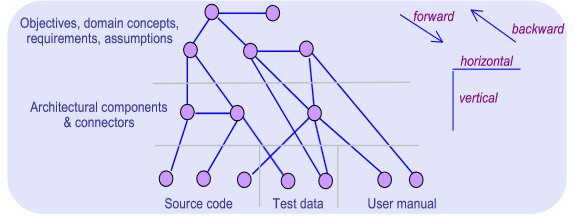
\includegraphics[width=\textwidth]{img/requirements/traceability-diagram.png}
      \caption{Traceability diagram}
      \label{fig:traceability-diagram}
\end{figure}

La backward traceability viene usata per stabilire perché un certo elemento sia
lì e da dove viene (anche ricorsivamente) mentre la forward per stabilire dove un
elemento verrà considerato e con quali implicazioni (anche ricorsivamente).
Ricorsivamente perché posso andare indietro/avanti di più step. Bisogna localizzare
e valutare l'impatto dei cambiamenti lungo i collegamenti orizzontali/verticali.

Elencando le varie tecniche TM, per tracciare i vari collegamenti, si hanno:
\begin{itemize}
      \item Cross referencing
      \item Matrici di tracciabilità
      \item Feature diagrams (nel dettaglio quelli con supporto a più variant link
            type)
      \item Database di tracciabilità
      \item Database di modelli di tracciabilità
      \item Tracciabilità Specification-based
\end{itemize}
È comunque un discorso molto complesso, costoso e studiato.

Approfondiamo il cross referencing.

Con questa tecnica si seleziona ogni elemento da tracciare e gli si assegna un
nome unico. Si definisce poi lo schema di indice/tag per collegarli lessicalmente e
si configura un motore di ricerca su tale schema. Si recuperano quindi gli elementi
seguendo le catene di riferimenti incrociati, le cross-reference chains. Un esempio
banale in un documento potrebbe essere specificare che sezione dello stesso documento
andare a guardare per chiarire un certo concetto.

Come pro si hanno:
\begin{itemize}
      \item la leggerezza e la disponibilità
      \item il supporto di ogni livello di granularità (assegnando identificatori
            a ciò che vogliamo)
\end{itemize}
Come contro:
\begin{itemize}
      \item un solo tipo di collegamento, quello lessicale, privo di semantica
      \item informazioni di tracciabilità nascoste
      \item il costo del mantenimento dello schema di indicizzazione (anche se si ha
            un basso costo iniziale)
      \item controllo e analisi limitate
\end{itemize}
In merito alla \textbf{matrice di tracciabilità} \ref{fig:dependency-matrix} abbiamo che essa è la matrice
di adiacenza di un grafo a singola relazione di tracciabilità, detto \textbf{dependency graph}.
In posizione ($i,j$) troviamo 1 se si ha un arco orientato tra l'item $T_i$ e
l'item $T_j$ , 0 altrimenti. Possiamo quindi dire che sulla riga i-sima troviamo
gli elementi che dipendono da $T_i$ e sulla colonna i-sima gli elementi che sono
dipendenza di $T_i$.

Come pro si hanno:
\begin{itemize}
      \item Navigazione backward e forward
      \item Semplice analisi dello schema (ad esempio è semplice identificare un
            ciclo di dipendenza, avendo un ciclo nel grafo)
\end{itemize}
Come contro:
\begin{itemize}
      \item Grafi di grandi dimensioni sono soggetti ad errori oltre ad essere
            difficilmente gestibili
      \item Supportano un solo tipo di relazione
      \item Dovrei creare più matrici per collegamenti tra oggetti con semantiche
            diverse
\end{itemize}

\begin{figure}[!ht]
      \centering
      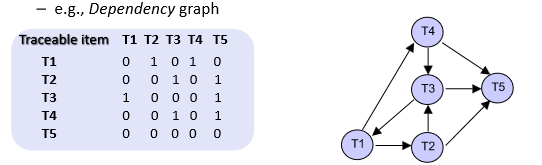
\includegraphics[width=\textwidth]{img/requirements/dependency-matrix.png}
      \caption{Dependency matrix}
      \label{fig:dependency-matrix}
\end{figure}

Quest'ultimo contro può essere risolto coi \textbf{feature diagrams} \ref{fig:feature-diagram} che sono
rappresentazione grafica dei punti in comune e delle varianti del sistema, permettendo
la rappresentrazione compatta di un gran numero di varianti. Avere più varianti
permette di distribuire il sistema con un ampio numero di feature.

Nel diagramma le feature sono rettangoli e possono essere obbligatorie (con un
pallino nero) o opzionali (con un pallino bianco). Si hanno anche potenziali or
esclusivi, or non-esclusivi e and per separare in diversi modi feature in sotto-feature.
Le varie combinazioni espresse dalle feature del digramma, seguendo la logica di
opzionali o meno e delle varie suddivisioni esprimono le varianti del progetto.

\begin{figure}[!ht]
      \centering
      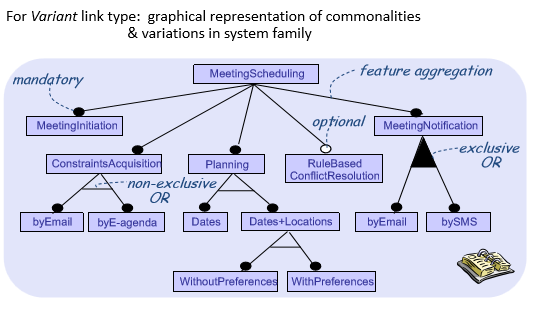
\includegraphics[width=\textwidth]{img/requirements/feature-diagrams.png}
      \caption{Feature diagram}
      \label{fig:feature-diagram}
\end{figure}
\chapter{Model-View-Controller}
Il \textbf{Model-View-controller} (\textbf{MVC}) è un pattern architetturale molto
diffuso nello sviluppo di sistemi software, in particolare nell'ambito della
programmazione orientata agli oggetti e in applicazioni web, in grado di separare
la logica di presentazione dei dati dalla logica di business. Partiamo analizzando
il pattern architetturale:
\begin{figure}[!ht]
      \centering
      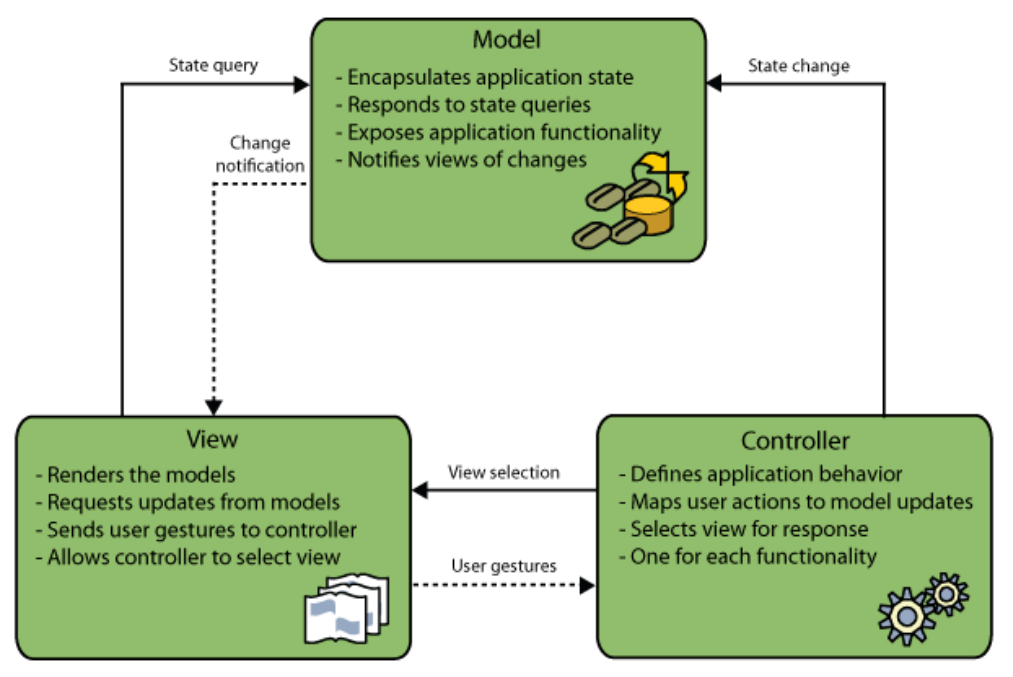
\includegraphics[width=0.5\textwidth]{img/mvc/mvcpattern.png}
      \caption{Model View Controller}
      \label{fig:enter-label}
\end{figure}
Dove con le frecce piene si hanno le invocazioni di metodi e con quelle
tratteggiate gli eventi. Analizzando meglio le tre componenti si ha che:
\begin{itemize}
      \item \textbf{Model}: incapsula lo stato dell'applicazione, fornisce i
            metodi per accedere ai dati utili dell'applicazione. È implementato
            dalle classi che realizzano la logica applicativa.
      \item \textbf{View}: renderizza il modello, richiede l'aggiornamento dai
            modelli, invia le operazioni dell'utente al \textit{controller} e gli
            permette di selezionare la vista. Visualizza i dati contenuti nel
            model e si occupa dell'interazione con utenti e agenti. Presenta lo
            stato del model all'utente.
      \item \textbf{Controller}: definisce il comportamento dell'applicazione,
            riceve i comandi dell'utente (in genere attraverso il \textit{View})
            e li attua modificando lo stato degli altri due componenti. Si ha un
            controller per funzionalità. È un mediatore tra view e controller.
\end{itemize}
La \textit{view} raccoglie gli input dell'utente e li inoltra al \textit{controller},
che li mappa in operazioni sul \textit{model}, che viene modificato. A questo punto
il controller seleziona la nuova view da mostrare all'utente, che a sua volta
interagisce per avere i dati con il model. Cambi del model sono notificati alla
view per eventuali cambiamenti dei dati.

Per la costruzione del controller si hanno vari design pattern tra cui:
\begin{itemize}
      \item \textbf{Page Controller}: si ha un controller per pagina che si
            occupa di:
            \begin{itemize}
                  \item Controllare i parametri delle richieste e richiamare la
                        business logic sulla base della richiesta.
                  \item Selezionare la view successiva da mostrare.
                  \item Preparare i dati per la presentazione.
            \end{itemize}
            Si ha il seguente flusso di controllo:
            \begin{enumerate}
                  \item Il controllo si sposta dal server Web al Page Controller.
                  \item Estrae i parametri dalla richiesta.
                  \item Utilizza alcuni oggetti di business.
                  \item Decide la view successiva.
                  \item Prepara i dati da mostrare nella view successiva.
                  \item Porta il controllo (e i dati) alla view.
            \end{enumerate}
            Dal punto di vista implementativo si possono usare soluzioni con poca
            logica di controllo o con una forte logica di controllo. Con questo
            pattern si implementa un controller per ciascuna pagina logica, avendo,
            per la scalabilità, la crescita finita del controller proporzionale
            al numero di pagine necessarie, producendo un numero comunque finito
            e gestibile di file di codice piccoli.
      \item \textbf{Front Controller}: definisce un singolo componente per gestire
            tutte le richieste. Ogni volta che si riceve una richiesta, il front
            controller rappresentato dall'\textbf{handler} si avvale della
            collaborazione di una gerarchia di classi, le quali rappresentano i
            comandi che possono essere richiesti dall'utente attraverso
            l'interfaccia. Questo approccio risulta scalabile perché al crescere
            della dimensione dell'applicazione ciò che cresce non è l'handler ma
            cresce la gerarchia dei comandi. Nel dettaglio l'handler:
            \begin{itemize}
                  \item Riceve la richiesta dal server.
                  \item Esegue operazioni generali/comuni a tutti i comandi.
                  \item Decide l'operazione che deve essere eseguita e alloca
                        l'istanza del comando.
                  \item Delega l'esecuzione al comando istanziato.
            \end{itemize}
            mentre il comando:
            \begin{itemize}
                  \item Estrae i parametri dalla richiesta.
                  \item Invoca metodi implementati nella business logic.
                  \item Determina la vista successiva.
                  \item Dà il controllo al View.
            \end{itemize}
            Il front controller è più complesso del page controller. Inoltre evita
            la duplicazione del codice tra i vari controller, permette una semplice
            configurazione del server avendo una sola servlet, permette di gestire
            dinamicamente nuovi comandi, facilita l'estensione del controller e
            i comandi possono essere implementati sia come metodi, sia come classi.
            Al crescere dell'applicazione cresce la gerarchia di comandi, mantenendo
            quasi invariato il front controller.
      \item \textbf{Intercepting Filter}: è utile per gestire richieste e risposte
            prima che vengano servite. Viene spesso usato insieme al front
            controller per “decorare” richieste e risposte con funzioni aggiuntive.

            Dal punto di vista implementativo il web server fornisce Filter Manager
            e Filter chain, dovendo quindi implementare e dichiarare solo i filters.
            \begin{figure}[!ht]
                  \centering
                  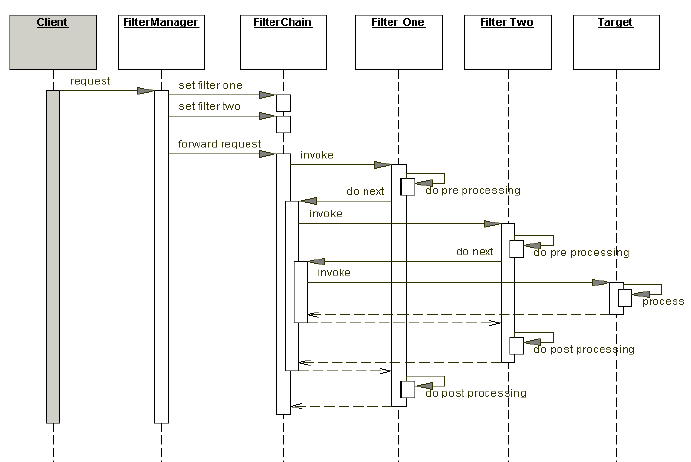
\includegraphics[width=0.5\textwidth]{img/mvc/filter.png}
                  \caption{Comportamento del Intercepting Filter}
            \end{figure}
            I filtri sono composti da:
            \begin{itemize}
                  \item \textbf{preprocessing}: operazioni prima delle invocazioni.
                  \item \textbf{invocazione}: si invocano le funzionalità della
                        filter chain.
                  \item \textbf{postprocessing}: operazioni dopo le invocazioni.
            \end{itemize}
      \item \textbf{Application Controller}: usato in quanto all'aumentare della
            complessità del flusso, la gestione del flusso potrebbe essere
            concentrata in una classe. Solitamente viene usato dal page controller
            o dal front conteoller.
\end{itemize}
Possiamo definire anche i design pattern per l'implementazione della view:
\begin{itemize}
      \item \textbf{Template View}: che genera codice HTML dalle pagine template
            che includono chiamate al modello. Dove nel codice HTML si hanno vari
            marker e l'\textbf{helper} genera i dati del dominio e separa la vista
            dalla logica di implementazione.

            L'helper è creato dal controller ed è accedibile da una vista. Si usano
            anche i metodi helper del controller per recuperare i dati dal Model,
            permettendo di preparare dei dati ad hoc per la parte di presentazione,
            tramite getter specifici.
      \item \textbf{Transformation View}: che trasforma le entità di dominio in
            HTML. Dove per il model tipicamente ogni classe implementa un metodo
            \textit{.toXML()} mentre per il transformer si ha tipicamente
            l'implementazione tramite \textit{eXtensible Style Language for
                  Transformations} (XSLT). Si ha quindi che ci si concentra
            sull'entità che deve essere trasformata, piuttosto che sulla pagina
            di output. Si ha una produzione interamente dinamica della pagina da
            parte del transformer. Il trasformer legge la conversione XML e le
            regole XSLT, crea la pagina dinamicamente, inserendo i dati del model
            definito come XML nel posto specificato dalle regole XSLT.

            Purtroppo è difficile includere la logica di implementazione nella view
            anche se il testing è facile. È facile da applicare a dati in formato
            XML anche se What You See Is What You Get (WYSIWYG) sarebbe più intuitivo
            e facile da implementare. Al contrario di template view non vediamo
            cosa stiamo facendo fino a che non visualizziamo. Template view è usato
            spesso per costruire solo parti di pagine.
      \item \textbf{Two-Steps View} dove si ha la generazione della pagina HTML
            in due passaggi:
            \begin{enumerate}
                  \item Si genera un pagina logica.
                  \item Si renderizza la pagina.
            \end{enumerate}
            Spesso collassano in un'unica fase.

            Dal punto di vista implementativo si può implementare secondo due
            metodologie:
            \begin{itemize}
                  \item 2 passi XSLT: Una sequenza di due trasformazione XSLT,
                        la prima per la costruzione della pagina logica e la
                        seconda per il suo render.
                  \item template-view: Una vista template con tag custom, la pagina
                        HTML è quindi la pagina logica e i tag custom il render.
            \end{itemize}
            Si ha che il “Look \& Feel” è facile da cambiare perché il rendering
            non è ottenuto tramite interazione con la strutturazione delle
            informazioni che devono essere visualizzate nella pagina.
\end{itemize}
\section{Object Relational Mapping}
Come sappiamo non si ha una relazione diretta tra programmazione a oggetti e
modello relazionale. Per questo si usa l'\textbf{Object Relational Mapping}
(\textbf{ORM}) quando si lavora con la programmazione a oggetti e dati persistenti
in un database con le classi che vanno \textit{mappate} nelle entità e viceversa.
Molti dei concetti si applicano ad altri mapping con modelli anche NoSQL. Si sfrutta
quindi un \textbf{API gateway} tra il client e le risorse dati che “incapsula”
l'accesso a una risorsa esterna con una classe e traduce le richieste di accesso
alla risorsa esterna in chiamate all'API. Con questo approccio si nasconde l'accesso
alle risorse e la complessità delle API.

Si hanno tipicamente 4 pattern per il database gateway:
\begin{itemize}
      \item \textbf{Table Data Gateway}: che prevede un oggetto per tabella. Prevede
            classi stateless ed è comodo nel paradigma procedurale ma meno in
            quello ad oggetti, in quanto i metodi ritornano dati row e non oggetti.
      \item \textbf{Row Data Gateway}: che prevede un oggetto per record. Si possono
            avere più copie di oggetti persistenti in memoria, avendo una classe
            gateway che funge da alter-ego del database che viene chiamata dalla
            classe coi metodi finder.
      \item \textbf{Active Record}: che prevede un oggetto per record.
      \item \textbf{Data Mapper}: che prevede un layer applicativo dedicato all'ORM.
\end{itemize}
\subsection{Active record}
Considerate le classi che implementano i dati che devono essere persistenti si
arricchiscono le classi con metodi per permettere l'interazione col database. Un
\textbf{active record} include quindi:
\begin{itemize}
      \item La business logic.
      \item Il mapping logico al database, avendo  metodi statici come \textit{finder}
            (invocabili avendo accesso alla classe) che comunque restituiscono
            risultati già nel dominio (oggetti o collezioni di oggetti) e non
            statici i metodi gateway per lavorare con le istanze.
\end{itemize}
Tra i metodi abbiamo quindi:
\begin{itemize}
      \item \textbf{Load}: che crea un'istanza a partire dai risultati di una query
            SQL. Potrebbe essere necessario creare altri oggetti con accesso a
            più tabelle nel casi di reference.
      \item \textbf{Costruttore}: per creare nuove istanze che saranno poi rese
            persistenti invocando metodi appositi.
      \item \textbf{Finder} (statici): che incapsulano la query SQL e ritornano
            una collezione di oggetti.
      \item \textbf{Write}: tra cui si hanno:
            \begin{itemize}
                  \item \textbf{Update}: per aggiornare un record a seconda dei
                        valori degli attributi.
                  \item \textbf{Insert}: per aggiungere un record a seconda dei
                        valori degli attributi.
                  \item \textbf{Delete}: per cancellare il record corrispondente
                        all'oggetto in analisi.
            \end{itemize}
            serve sincronizzazione tra oggetto in memoria ed entità nel database.
            Per farlo si ha un attributo identificatore nella classe che compare
            anche nel record e che serve per trovare il record corrispondente ad
            un oggetto.
      \item \textbf{Getter} e \textbf{Setter}: che a seconda del caso devono essere
            subito sincronizzati con il database.
      \item \textbf{Business}.
\end{itemize}
Non è il metodo migliore dal momento che nella stessa classe ho sia i metodi
della logica di business, sia i metodi per il mapping nel database. In aggiunta,
forza anche la corrispondenza perfetta tra OOP e ER design. Il lato positivo è la
semplicità.
\subsection{Data mapper}
Con il pattern \textbf{Data Mapper} invece si ha un layer software indipendente,
dedicato alla persistenza e all'ORM, in modo che la logica di dominio non conosca
la struttura del database e nemmeno le query SQL. Si usano quindi interfacce per
consentire l'accesso ai mapper indipendentemente dalla loro implementazione.

Framework moderni implementano questo tipo di pattern (che offre la parte di
mapping senza doverli implementare, a solo configurare).
\subsection{Ulteriori pattern ORM}
In generale si hanno dei pattern di comportamento per risolvere altri problemi ORM:
\begin{itemize}
      \item \textbf{Unit of work}
      \item \textbf{Identity map}
      \item \textbf{Lazy load}
\end{itemize}
e anche pattern strutturali:
\begin{itemize}
      \item \textbf{Value holder}
      \item \textbf{Identify field}
      \item \textbf{Embedded value}
      \item \textbf{LOB}
\end{itemize}
\subsubsection{Unit of work}
In questo caso si approfondiscono le operazioni ACID cercando di capire quando
sincronizzare le informazioni in memory con il database. Questo aspetto è importante
introducendo il concetto di \textbf{business transaction} per operazioni con
semantica di tipo all or nothing dove o si accettano tutte le operazioni richieste
o nessuna. Le business transaction vanno quindi mappate nelle \textbf{system
      transaction} fatte dal sistema sul database.

Si hanno varie soluzioni:
\begin{itemize}
      \item \ref{fig:bt-uguale-st} aggiornare il database ogni volta che si ha
            una modifica in memoria. Si lega la business transaction con la system
            transaction. Infattibile perché si avrebbe che la transazione del DB
            sarebbe troppo lunga, comportando che l'aggiornamento impedisce
            l'accesso agli altri.
            \begin{figure}[!ht]
                  \centering
                  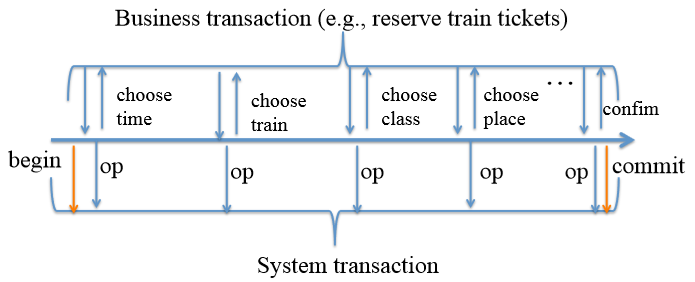
\includegraphics[width=0.5\textwidth]{img/mvc/bt-uguale-st.png}
                  \caption{System transaction uguale alla Business transaction}
                  \label{fig:bt-uguale-st}
            \end{figure}
      \item \ref{fig:op-uguale-st} aggiornare il database ad ogni modifica in
            memoria. Per la business transaction si hanno tante system transaction
            una per ogni modifica. Si rischia inconsistenza perché si hanno
            diversi aggiornamenti ma in periodi diversi.
            \begin{figure}[!ht]
                  \centering
                  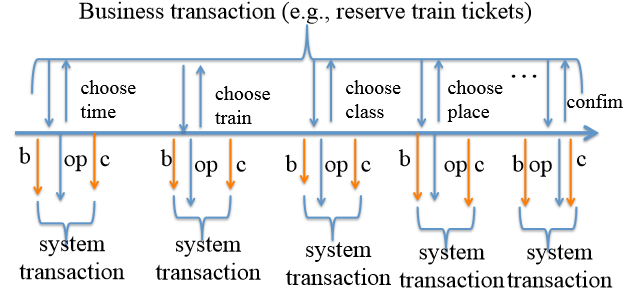
\includegraphics[width=0.5\textwidth]{img/mvc/op-uguale-st.png}
                  \caption{System transaction per ogni singola operazione nella Business
                        transaction}
                  \label{fig:op-uguale-st}
            \end{figure}
      \item \ref{fig:bt-uguale-st1} aggiornamento finale al termine della business
            transaction.
            \begin{figure}[!ht]
                  \centering
                  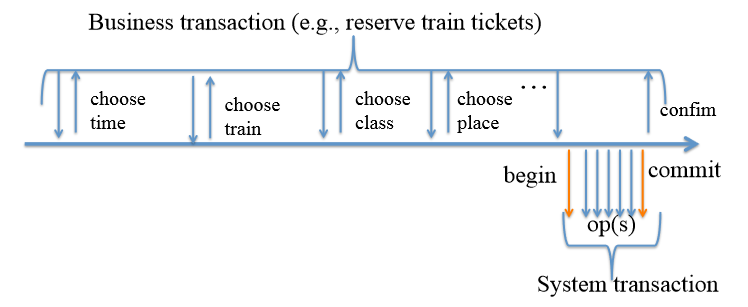
\includegraphics[width=0.5\textwidth]{img/mvc/st-finale.png}
                  \caption{System transaction alla fine della Business transaction}
                  \label{fig:bt-uguale-st1}
            \end{figure}
\end{itemize}
La \textbf{unit of work} quindi traccia ogni cambiamento (coi metodi register) e
lo attuta in una singola system transaction finale (con il commit). Per fare questo
incapsula ogni update/insert/delete, mantenendo l'integrità del database ed
evitando deadlock.

A proposito di \textit{locking} si ha che due business transaction possono essere
attive nello stesso momento e bisogna capire come devono lavorare sul database.
In questo caso si hanno due strategie:
\begin{itemize}
      \item \textbf{Optimistic locking}: usato quando si hanno poche probabilità
            di generare conflitti, avendo diversi utenti che lavorano spesso su
            dati differenti, e si bassa su un numero che identifica la versione
            degli oggetti registrati. Due business transaction possono quindi
            interferire accedendo e modificando i record ma si sfrutta il numero
            di versione per tenere traccia delle modifiche e se una transazione
            vede che il numero di versione di un record è incrementato e in tal
            caso si ricarica il record tramite un rollback.
      \item \textbf{Pessimistic locking}: usato quando hanno alte probabilità di
            generare conflitti. Gli oggetti sono bloccati non appena vengono
            usati riducendo la concorrenza. Non si permette quindi alle transazioni
            di lavorare concorrentemente riducendo però le prestazioni del sistema
            ma aumentando la sicurezza.
\end{itemize}
Poi, per avvisare la unit of work che un'operazione di persistenza è stata
schedulata, si hanno due pattern:
\begin{itemize}
      \item \textbf{Caller registration}: dove chi modifica l'entità lo notifica
            direttamente alla unit of work. Questa soluzione è rischiosa in quanto
            il programmatore potrebbe dimenticarsi ma permette maggior flessibilità,
            permettendo di decidere dinamicamente se i cambiamenti devono
            “riflettersi” sullo storage persistente.
      \item \textbf{Object registration}: dove è l'entità modificata a notifica la
            unit of work, che però deve obbligatoriamente avere accesso globale.
            Ogni cambiamento viene comunque notificato. Solitamente si usa questa
            soluzione ma nella variante in cui le classi persistenti non includono
            il codice per la notifica ma tramite una strumentazione trasparente
            offerta dai framework.
\end{itemize}
\subsubsection{Identity map}
In questo caso si studia il load di un'istanza direttamente a partire dal database.
Se un certo record viene richiesto due volte si generano due oggetti uguali.
In pratica uno stesso oggetto può essere caricato più volte, o da azioni differenti
dello stesso utente rischiando inconsistenze, se una istanza viene modificata,
oltre ad avere ridondanza di dati o da utenti diversi in questo spesso è intenzionale.

\textbf{Identity map} è quindi un oggetto con la responsabilità di identificare
gli oggetti caricati in una sessione, funzionando come una sorta di cache,
controllando l'eventuale presenza dell'oggetto “in cache” prima di caricarne uno
nuovo, se già presente si ritorna un riferimento all'oggetto. Identity map quindi
mantiene i riferimenti agli oggetti tramite un sistema chiave-valore.

Generalmente la chiave della mappa è quella primaria del database. Si hanno
diverse identity map:
\begin{itemize}
      \item Una per applicazione, se chiavi di entità differenti sono disgiunte.
      \item Una per classe.
      \item Una per tabella, generalmente meglio se una per classe.
\end{itemize}
\subsubsection{Lazy load}
A volte è necessario avere solo una parte di un oggetto per eseguire una certa
operazione anche perché alcuni attributi possono essere particolarmente pesanti.
Si parla quindi di efficienza.

Si procede quindi con il pattern lazy load che crea oggetti inizializzando solo
alcuni attributi lasciando comunque possibilità si caricare in seguito ulteriori
attributi non ancora inizializzati se ce ne fosse necessità, in modo on-demand,
tramite i finder.
\subsubsection{Value holder}
Con questa tecnica si usa un oggetto, il value holder, come uno storage
intermediario per un attributo. Anche in questo caso si ha un'inizializzazione
“lazy” implementata da questo oggetto che caso per caso potrebbe essere istanziato
con diverse strategie di load. Si separa la locgia di dominio da quella “lazy”
di loading.
\subsubsection{Identify field}
Normalmente si hanno:
\begin{itemize}
      \item L'identità in memory rappresentata dalla reference dell'oggetto.
      \item L'identità nel database rappresentata dalla chiave primaria.
\end{itemize}
e si ha bisogno di accoppiare/sincronizzare le due identità per la consistenza
dei dati.

La soluzione è usare l'identity field ovvero un “nuovo” attributo nell'oggetto
il cui valore diventa la “chiave primaria” (solitamente chiamato id, di tipo long).
Non si usano i normali attributi/identificatori della classe perché potrebbero
modificare nel tempo di sviluppo del programma.

Si hanno infatti due tipi di chiave:
\begin{itemize}
      \item Una chiave derivata da attributi dell'oggetto (che sono usati anche
            dall'applicazione). Si ha comunque rischio di duplicazione, avere
            assenza di valore e avere cambiamenti sulla logica di dominio che
            impattano su quella di persistenza.
      \item Chiavi dedicate, sia semplici (un solo attributi) che composte (di più
            attributi), avendo una chiave per tabella e una per database.
            Nella pratica spesso hanno tipo long che ben supporta il check di
            uguaglianza (==) e la generazione di nuove chiavi.
\end{itemize}
Si hanno varie strategie per la generazione delle chiavi:
\begin{itemize}
      \item Direttamente dal database (con sequenze o id delle colonne).
      \item Tramite GUID, ovvero Globally Unique IDentifier, tramite opportuni
            software e libreria.
      \item Dall'applicazione, principalmente in due modi:
            \begin{itemize}
                  \item \textbf{Table scan}, usando una query SQL per determinare
                        il valore della prossima chiave.
                  \item \textbf{Key table}, usando tabelle speciali con il nome
                        delle altre tabelle e il valore successivo della chiave.
            \end{itemize}
\end{itemize}
I moderni framework ORM supportano i vari design pattern appena discussi e quelli
mancanti, relativi a chiavi esterne, cascading, ereditarietà $\dots$ In ogni caso
i pattern appena discussi sono tutti supportati dai moderni framework ORM.
\subsubsection{Embedded value}
Con questo pattern si hanno semplici oggetti, senza un chiaro concetto di identità,
che possono essere inclusi in oggetti che fungono da alter-ego delle tabelle
anziché creare tabelle dedicate.
\subsection{JPA}
\textbf{Java Persistence API} (JPA) è unos standard di implementazione di ORM nel
linguaggio Java. Questa implementazione consiste in un grande set di pattern/
meccanismi già implementati mediante:
\begin{itemize}
      \item Sistema di annotazioni.
      \item Servizio.
\end{itemize}
Si hanno 4 macroelementi:
\begin{itemize}
      \item \textbf{Database}: che salverà degli oggetti, istanze di entity class,
            classi con un mapping ad un record. Il mapping è garantito attraverso
            le annotazioni.
      \item Classi della logica di dominio.
      \item \textbf{Entity manager}: servizio che permette di lavorare sulle entità
            persistenti
\end{itemize}
\subsubsection{Entity manager}
Gli oggetti persistenti sono anche chiamati come \textbf{Pojo} (\textit{Plain Old
      Java Objects}) perché oggetti normali Java ma con annotazioni. Sono uguali
fino a quando non interagiscono con l'entity manager.

Ogni Pojo in memoria può trovarsi in 2 stati:
\begin{itemize}
      \item \textbf{managed}: entity manager è consapevole nella presenza in memoria.
      \item \textbf{unmanaged}: entity manager non è consapevole nella presenza
            in memoria.
\end{itemize}
Essenziale lo stato per implementare il pattern Unit of Work e Identity map.
In caso di creazione o cancellazione di entità dobbiamo notificarlo alla Unit of
Work mentre nel caso di modifica queste vengono applicate automaticamente.
Entity Manager cattura le notifiche e c'è una trasparenza nella notifica.

Un'entità diventa managed quando si crea da una classe con annotazione
\textit{entity}, mentre è considerata unmanaged quando viene scambiata tra diverse
parti. In questo caso bisogna notificarlo all'Entity Manager.

Il servizio Entity Manager è in grado di gestire solo le classi che dichiariamo
(insimee di classi persistenti = persistence unit) e vengono dichiarati nel file
persistence.xml e si deve specificare una connessione al database. A runtime la
persistence unit si chiama persistence context. (si possono dichiarare più
persistence unit e context)

L'annotazioen @Entity specifica un oggetto persistente e avremo una tabella
per memorizzare gli oggetti con le colonne con gli stessi nomi degli attributi.
Si possono utilizzare annotazioni per modificare il mapping come i nomi dei fields
e delle tabelle.

Definito il mapping utilizzeremo Entity Manager per accedere ai dati. Creiamo
l'Entity Manager e per notificare la creazione si usa la funzione di persist.
(UoW) La scrittura non è immediata perché aspetta quando si aprirà la transazione.
Dall'Entity Manager posso recuperare l'entità con i metodi finder che chiedono la
classe dell'oggetto richiesto e id. Il risultato dei metodi sono sempre oggetti.
getReference è caricamento Lazy.
Un altro modo di estrazione degli oggetti è attraverso una query simile a SQL, non
si usano i nomi delle tabelle o field delle tabelle ma bensì ai nomi delle classi
e attributi (sempre secondo object oriented).
Per modificare le entità si modificano gli attributi e alla prossima transazione
verrà salvata in automatico. La modifica non viene riportata al database se l'entità
è unmanaged. Per renderla effettiva allora si usa merge che:
\begin{itemize}
      \item se l'entità non esiste allora viene inserita.
      \item se esiste un'altra entità si sovrascrive l'unmanaged sul database.
\end{itemize}

refresh posso aggiornare l'entità

per aprire e chiudere la transaction ci sono dei metodi dell'Entity Manager.

SequenceGen(nome generatore in Java, nome generatore nel DB)

Cerca di usare sempre un'attributo ad hoc per le chiavi.

Possiamo fare il mapping di un'entità su più tabelle con SecondaryTable e l'entità
sarà partizionata tra le due tabelle che hanno i record associati con lo stesso id.
Utile per accedere a database legacy e codificare più tabelle in un'entità.

Mapping delle associazioni comportano il caricamento anche delle entità associate.
Vediamo ora come implementare le associazioni:
\begin{itemize}
      \item \textbf{One-to-One} monodirezionale: si hanno due modi per mappare
            una relazione 1 a 1:
            \begin{enumerate}
                  \item Utilizzando una chiave esterna nella tabella padre che punta
                        alla tabella figlia.
                  \item Effettuando la join sulle chiavi primarie, in questo modo si
                        ha un entità suddivisa in due tabelle.
            \end{enumerate}
      \item \textbf{One-to-Many} monodirezionale: nella parte a 1 si memorizza
            una collection della parte a molti. Questo può essere gestito con una
            tabella di join, specificando il nome della tabella e le chiavi da
            utilizzare.
      \item \textbf{Many-to-One} monodirezionale: si applica lo stesso ragionamento
            della one-to-many invertendo i ruoli.
      \item \textbf{Relazioni bidirezionali}: sono raramente utilizzate. Si possono
            creare aggiungo un campo in entrabe le classi e specificando in una
            delle due entità il mapping al campo della classe a cui fare riferimento.
      \item \textbf{Many-to-Many}: si crea una tabella di join utilizzando le
            chiavi primarie delle due entità. Nelle classi è possibile esprimere
            un campo di tipo collection che rappresenta gli elementi dell'altra
            classe che partecipano alla relazione.
\end{itemize}

Utilizzando questo approccio si progettano direttamente le classi e non il database.

Dato che nella programmazione a oggetti posso avere delle gerarchie tra gli oggetti,
ma questi non sono supportati dal modello relazionale, si ha la necessità di mappare
le gerarchie. Il mapping deve essere fatto in modo esplicito:
\begin{itemize}
      \item \textbf{Single table}: tutto in una tabella e si introduce un attributo
            discriminatore. Richiede che sia possibile avere null negli attributi.
            Veloce e semplice ma si vincola ad non avere not null.
      \item \textbf{1 tabella per classe}: dove ogni classe ha una tabella
            associata con un campo per ogni attributo. Tutti gli attributi di una
            classe sono quindi in una singola tabella dedicata. Si ha un maggior
            controllo dei vincoli e un mapping ancora semplice ma è difficile
            da gestire con l'Entity Manager e il DBMS deve supportare la SQL
            UNION.
      \item \textbf{1 tabella per sottoclasse}: dove si ha una classe per tabella
            ma senza una copia degli attributi per le classi figlie, le quali sono
            caratterizzate solo dall'id e dagli attributi extra rispetto alla
            classe padre. Si ha quindi un mapping “uno a uno”. Questa strategia
            supporta i vincoli tabellari e non richiede la SQL UNION ma si ha un
            istanza “splittata” su più tabelle ed è generalmente una soluzione
            lenta in esecuzione (dovendo eseguire i join).
\end{itemize}
Si mappa Ereditarietà perché permette di ridurre la duplicazione e di risolvere
le query correttamente.
\section{Gestione delle dipendenze}
Vogliamo sviluppare codice in classi che siano il più indipendenti possibili e con
più disaccoppiamento possibile, si può considerare ciascuna classe come un singolo
componente, le quali possono essere componibili tra di loro per risolvere un problema
o implementare un servizio. Mantenendo l'indiependenza tra i componenti del sistema
si introduce una semplicità nella fase di manutenzione e evoluzione del sistema.

Le dipendenze tra i componenti possono essere soddisfatte in due modi:
\begin{itemize}
      \item \textbf{Dinamicamente}: a runtime i componenti indipendenti vengono
            collegati, quindi si ha alto disaccoppiamento.
      \item \textbf{Staticamente}: si inserisce all'interno del componente parte
            del codice del compoente dipendente, in questo caso si ha una mancanza
            di disaccoppaimento perché la classe sarà meno riutilizzabile, dal
            momento che, esportandola, esporteremo anche la classe dipendente.
\end{itemize}
Nella gestione delle dipendenze un aspetto fondamentale è il \textbf{decoupling},
ovvero si rendono indipendeti le componenti da pubblicare anche se a runtime tali
componenti devono comunque interagire.

Si hanno quindi alcuni design pattern per gestire le dipendenze dinamicamente:
\begin{itemize}
      \item \textbf{Inversion control}: si ha un elemento esterno che definisce
            il valore della dipendenza, servizio che riempie i riferimenti
            dall'esterno (dependency injection).
      \item \textbf{Service locator}: si implementa un componente che gestisce
            le dipendenze per accedere ai componenti, in questo caso i riferimenti
            non vengono risolti in modo automantico, ma sarà il componente che
            manualmente farà richiesta al servizio di registry che ritornerà il
            componente cercato.
\end{itemize}
\subsection{Inversion control (Dipendency Injection)}
Si utilizza un componente esterno, chiamato \textbf{assembler} che si occupa di
connettere i componenti in automatico a runtime senza una loro effettiva richiesta.

La dipendenza viene risolta, attraverso l'assembler, alla creazione dell'oggetto
in modo trasparente. Questa operazione può essere fatta tramite:
\begin{itemize}
      \item \textbf{Costruttore}: si ha un attributo della classe che rappresenta
            la dipendenza e lo si inizializza attraverso il costruttore.
      \item \textbf{Metodi setter}: si ha un attributo della classe che rappresenta
            la dipendenza e lo si inizializza attraverso uno specifico metodo
            setter.
      \item \textbf{Interfacce}: si ha un attributo della classe e un'interfaccia
            che dichiara il setter, l'assembler utilizza il metodo setter definito
            nell'interfaccia per risolvere la dipendenza. (utilizzata raramente)
      \item \textbf{Reflection}: non si utilizza un metodo ma bensì le annotazioni.
            In Java, si utilizza @Autowired la quale specifica che deve essere
            risolta la dipendenza e con @Component che specifica cosa utilizzare
            per riempire gli Autowired.
\end{itemize}
Generalmente l'assembler viene fornito dal framework e può essere configurato
utilizzando un file di configurazioni o attraverso delle annotazioni.
\begin{figure}[!ht]
      \centering
      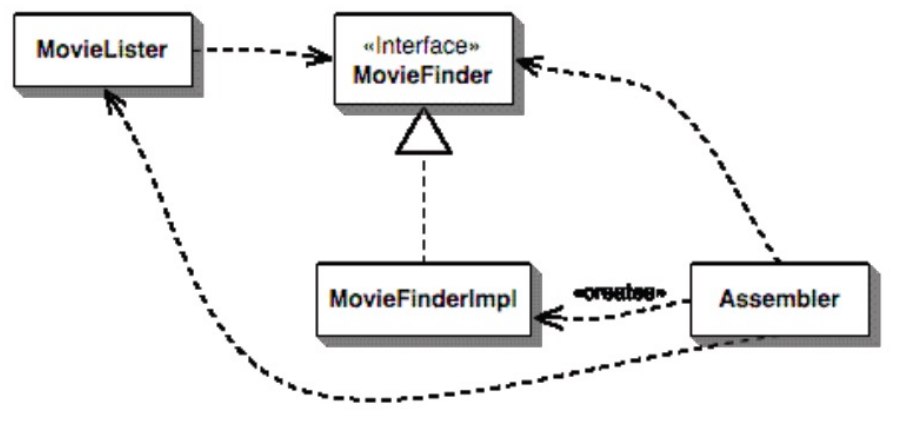
\includegraphics[width=0.5\textwidth]{img/mvc/inversion-control.png}
      \caption{Inversion control implementation}
\end{figure}
\subsection{Service locator (Dependency lookup)}
Si utilizza una classe che implementa servizio di locazione, solitamente si realizza
utilizzando una classe singleton la quale contiene una mappa chiave-valore che
tiene traccia dei componenti instanziati.

In sostanza si definiscono i singoli componenti che implementano un'interfaccia
factory. Quando noi definiamo i servizi si definisce un attributo del tipo del
factory che verrà associato attraverso reflection.

A questo punto la classe che deve soddisfare la dipendenza fa un accesso al service
locator chiedendo che venga ritornato un riferimento al componente che deve essere
utilizzato.

Quando si chiama il componente si utilizza il factory che fa la chiamata al lookup.
\section{Transaction}
Importante sarà definire le transazioni quando si accede al database, questo può
essere fatto attraverso le dichiarazioni specificate con le annotazioni.

Il ciclo vita delle transazioni è il seguente:
\begin{itemize}
      \item \textbf{inizio}: iniziano con la chiamata di un metodo che ha un'annotazione
            di apertura della transazione.
      \item \textbf{fine}: finiscono con la chiamata di un metodo che ha un'annotazione
            di chiusura della transazione.
\end{itemize}
In questo modo si separa la logica transazionale dalla logica di business perché
la prima viene gestita dal framework attraverso le annotazioni. Le annotazioni
transazionali si possono applicare alla classe (i metodi e attributi ereditano
l'annotazione) oppure a livello di metodo e attributo della classe. Se si specifica
l'annotazione a livello di classe, allora le annotazioni a livello di metodo saranno
un override di quella della classe.

Esistono vari tipi di annotazioni:
\begin{itemize}
      \item \textbf{Not supported}: il codice eseguito non fa parte della transazione.
      \item \textbf{Supports}: dipende dal chiamante, se c'è una transazione in
            corso anche il codice del metodo comparirà nella transazione, altrimenti,
            se non c'è la transazione allora il codice non appartiene alla transazione.
      \item \textbf{Required}: richiede che deve essere presente una transaction,
            se il chiamante non è in una transazione allora si avvia una nuova
            transazione, al contrario usa quella del chiamante.
      \item \textbf{RequiresNew}: crea una nuova transaction ad hoc per l'esecuzione.
      \item \textbf{Mandatory}: il codice deve essere eseguito in una transaction
            del chiamante, se il chiamante non ha attivato una transaction allora
            viene generata un'eccezione.
      \item \textbf{Never}: non deve mai essere eseguito il codice in una transazione,
            se il chiamante ha attivato una transazione allora questo ritorna
            un'eccezione.
\end{itemize}
Parlando di persistenza e transazioni parliamo anche di isolation e database
locking, ovvero quando si creano transazioni non necessariamente sono perfettamente
“isolate”. L'isolation può essere configurato per permettere un certo livello di
interferenza con la creazione temporanea di oggetti da parte di transazioni non
ancor concluse ma che possono essere letti da altre transaction. Se si modella
erroneamente la semantica transazionale allora si può avere:
\begin{itemize}
      \item \textbf{Dirty reads}: vengono letti i dati modificati da una transaction
            non ancora terminata, quindi si possono leggere dati che potrebbero
            non essere scritti sul database.
      \item \textbf{Unrepeatible reads}: transazioni che leggono lo stesso valore
            nella stessa transazione possono ritornare valori diversi. Questo
            può essere dovuto dal fatto che una transazione legge la stessa cosa
            ma tra le due letture c'è una \textit{modifica} del valore.
      \item \textbf{Phantom reads}: transazioni effettuano due letture, la seconda
            legge nuovi record che vengono \textit{inesriti} da una transazione
            tra le due.
\end{itemize}
Questo può essere risolto a livello di DBMS specificando le seguenti tipologie
di isolazioni:
\begin{itemize}
      \item \textbf{Read uncommitted}: si hanno dirty reads, unrepeatible reads e
            phantom reads.
      \item \textbf{Read committed}: si hanno unrepeatible reads e phantom reads.
      \item \textbf{Repeatable read}: si ha phantom reads.
      \item \textbf{Serializable}: isolation perfetta.
\end{itemize}
Si può definire l'isolation a livello di codice con annotazioni. La scelta del livello
di isolation comporta:
\begin{itemize}
      \item \textbf{Forte indipendenza}: performance basse perché si perde
            concorrenza
      \item \textbf{Bassa indipendenza}: performance alte perché si ha
            concorrenza.
\end{itemize}
\end{document}